\section{Simulation Analysis}
\label{sec:simulation}

\subsection{Operating Point Analysis}

Table~\ref{tab:op} shows the simulated operating point results for the circuit
under analysis. When compared to the theoretical analysis results, we see the same values
up to the 5 decimal places provided by ngspice.

\begin{table}[H]
  \centering
  \begin{tabular}{|l|r|}
    \hline    
    {\bf Name} & {\bf Value [A or V]} \\ \hline
    @ca[i] & 0.000000e+00\\ \hline
@gb[i] & -2.53212e-04\\ \hline
@r1[i] & 2.414774e-04\\ \hline
@r2[i] & 2.532123e-04\\ \hline
@r3[i] & -1.17349e-05\\ \hline
@r4[i] & -1.20106e-03\\ \hline
@r5[i] & -2.53212e-04\\ \hline
@r6[i] & 9.595831e-04\\ \hline
@r7[i] & 9.595831e-04\\ \hline
v(1) & 5.136122e+00\\ \hline
v(2) & 4.884647e+00\\ \hline
v(3) & 4.361951e+00\\ \hline
v(5) & 4.920010e+00\\ \hline
v(6) & 5.690271e+00\\ \hline
v(8) & -2.94454e+00\\ \hline
v(71) & -1.96654e+00\\ \hline
v(72) & -1.96654e+00\\ \hline

  \end{tabular}
  \caption{Operating point. A variable preceded by @ is of type {\em current}
    and expressed in Ampere; other variables are of type {\it voltage} and expressed in
    Volt.}
  \label{tab:p1}
\end{table}

\begin{table}[H]
    \centering
    \begin{tabular}{|l|r|}
      \hline    
      {\bf Name} & {\bf Value [A or V]} \\ \hline
      @gb[i] & -6.24390e-18\\ \hline
@r1[i] & 5.954528e-18\\ \hline
@r2[i] & 6.243896e-18\\ \hline
@r3[i] & -2.89368e-19\\ \hline
@r4[i] & 1.300919e-18\\ \hline
@r5[i] & -2.83857e-03\\ \hline
@r6[i] & -8.67362e-19\\ \hline
@r7[i] & 1.165891e-21\\ \hline
v(1) & 0.000000e+00\\ \hline
v(2) & -6.20107e-15\\ \hline
v(3) & -1.90901e-14\\ \hline
v(5) & -5.32907e-15\\ \hline
v(6) & 8.634810e+00\\ \hline
v(8) & 1.776357e-15\\ \hline
v(71) & 1.777545e-15\\ \hline
v(72) & 1.777545e-15\\ \hline

    \end{tabular}
    \caption{Operating point. A variable preceded by @ is of type {\em current}
      and expressed in Ampere; other variables are of type {\it voltage} and expressed in
      Volt.}
    \label{tab:p2}
  \end{table}

\subsection{Natural response}

  \begin{table}[H]
    \centering
    \begin{tabular}{|l|r|}
      \hline    
      {\bf Name} & {\bf Value [A or V]} \\ \hline
                                         Alínea 3 \\ \hline
                                   Transient Analysis  Wed Apr  7 17:26:26  2021\\ \hline
--------------------------------------------------------------------------------\\ \hline
Index   time            @ca[i]          @gb[i]          @r1[i]          \\ \hline
--------------------------------------------------------------------------------\\ \hline
0	0.000000e+00	0.000000e+00	0.000000e+00	0.000000e+00	\\ \hline
1	2.000000e-06	-2.83676e-03	8.921525e-16	-8.50806e-16	\\ \hline
2	4.000000e-06	-2.83496e-03	0.000000e+00	0.000000e+00	\\ \hline
3	8.000000e-06	-2.83135e-03	0.000000e+00	0.000000e+00	\\ \hline
4	1.600000e-05	-2.82414e-03	0.000000e+00	0.000000e+00	\\ \hline
5	3.200000e-05	-2.80978e-03	0.000000e+00	0.000000e+00	\\ \hline
6	6.400000e-05	-2.78129e-03	0.000000e+00	0.000000e+00	\\ \hline
7	1.280000e-04	-2.72516e-03	0.000000e+00	0.000000e+00	\\ \hline
8	2.280000e-04	-2.63971e-03	0.000000e+00	0.000000e+00	\\ \hline
9	3.280000e-04	-2.55695e-03	0.000000e+00	0.000000e+00	\\ \hline
10	4.280000e-04	-2.47677e-03	0.000000e+00	0.000000e+00	\\ \hline
11	5.280000e-04	-2.39912e-03	0.000000e+00	0.000000e+00	\\ \hline
12	6.280000e-04	-2.32389e-03	0.000000e+00	0.000000e+00	\\ \hline
13	7.280000e-04	-2.25103e-03	2.787976e-17	-2.65877e-17	\\ \hline
14	8.280000e-04	-2.18045e-03	0.000000e+00	0.000000e+00	\\ \hline
15	9.280000e-04	-2.11208e-03	0.000000e+00	0.000000e+00	\\ \hline
16	1.000000e-03	-2.06419e-03	-2.78798e-17	2.658770e-17	\\ \hline
17	1.010000e-03	-2.05764e-03	1.115191e-16	-1.06351e-16	\\ \hline
18	1.030000e-03	-2.04457e-03	1.115191e-16	-1.06351e-16	\\ \hline
19	1.070000e-03	-2.01868e-03	0.000000e+00	0.000000e+00	\\ \hline
20	1.150000e-03	-1.96789e-03	0.000000e+00	0.000000e+00	\\ \hline
21	1.250000e-03	-1.90619e-03	0.000000e+00	0.000000e+00	\\ \hline
22	1.350000e-03	-1.84642e-03	1.393988e-17	-1.32939e-17	\\ \hline
23	1.450000e-03	-1.78852e-03	1.393988e-17	-1.32939e-17	\\ \hline
24	1.550000e-03	-1.73245e-03	1.393988e-17	-1.32939e-17	\\ \hline
25	1.650000e-03	-1.67813e-03	0.000000e+00	0.000000e+00	\\ \hline
26	1.750000e-03	-1.62551e-03	0.000000e+00	0.000000e+00	\\ \hline
27	1.850000e-03	-1.57454e-03	0.000000e+00	0.000000e+00	\\ \hline
28	1.950000e-03	-1.52517e-03	0.000000e+00	0.000000e+00	\\ \hline
29	2.050000e-03	-1.47735e-03	0.000000e+00	0.000000e+00	\\ \hline
30	2.150000e-03	-1.43103e-03	0.000000e+00	0.000000e+00	\\ \hline
31	2.250000e-03	-1.38616e-03	0.000000e+00	0.000000e+00	\\ \hline
32	2.350000e-03	-1.34270e-03	1.393988e-17	-1.32939e-17	\\ \hline
33	2.450000e-03	-1.30060e-03	1.393988e-17	-1.32939e-17	\\ \hline
34	2.550000e-03	-1.25982e-03	0.000000e+00	0.000000e+00	\\ \hline
35	2.650000e-03	-1.22032e-03	0.000000e+00	0.000000e+00	\\ \hline
36	2.750000e-03	-1.18206e-03	1.393988e-17	-1.32939e-17	\\ \hline
37	2.850000e-03	-1.14499e-03	0.000000e+00	0.000000e+00	\\ \hline
38	2.950000e-03	-1.10909e-03	1.393988e-17	-1.32939e-17	\\ \hline
39	3.050000e-03	-1.07432e-03	0.000000e+00	0.000000e+00	\\ \hline
40	3.150000e-03	-1.04063e-03	0.000000e+00	0.000000e+00	\\ \hline
41	3.250000e-03	-1.00800e-03	0.000000e+00	0.000000e+00	\\ \hline
42	3.350000e-03	-9.76399e-04	6.969941e-18	-6.64693e-18	\\ \hline
43	3.450000e-03	-9.45784e-04	0.000000e+00	0.000000e+00	\\ \hline
44	3.550000e-03	-9.16129e-04	6.969941e-18	-6.64693e-18	\\ \hline
45	3.650000e-03	-8.87405e-04	0.000000e+00	0.000000e+00	\\ \hline
46	3.750000e-03	-8.59581e-04	6.969941e-18	-6.64693e-18	\\ \hline
47	3.850000e-03	-8.32629e-04	6.969941e-18	-6.64693e-18	\\ \hline
48	3.950000e-03	-8.06522e-04	0.000000e+00	0.000000e+00	\\ \hline
49	4.050000e-03	-7.81234e-04	6.969941e-18	-6.64693e-18	\\ \hline
50	4.150000e-03	-7.56739e-04	6.969941e-18	-6.64693e-18	\\ \hline
51	4.250000e-03	-7.33012e-04	6.969941e-18	-6.64693e-18	\\ \hline
52	4.350000e-03	-7.10028e-04	6.969941e-18	-6.64693e-18	\\ \hline
53	4.450000e-03	-6.87766e-04	0.000000e+00	0.000000e+00	\\ \hline
54	4.550000e-03	-6.66201e-04	0.000000e+00	0.000000e+00	\\ \hline
\\ \hline
Index   time            @ca[i]          @gb[i]          @r1[i]          \\ \hline
--------------------------------------------------------------------------------\\ \hline
55	4.650000e-03	-6.45313e-04	0.000000e+00	0.000000e+00	\\ \hline
56	4.750000e-03	-6.25079e-04	6.969941e-18	-6.64693e-18	\\ \hline
57	4.850000e-03	-6.05480e-04	0.000000e+00	0.000000e+00	\\ \hline
58	4.950000e-03	-5.86496e-04	0.000000e+00	0.000000e+00	\\ \hline
59	5.050000e-03	-5.68106e-04	0.000000e+00	0.000000e+00	\\ \hline
60	5.150000e-03	-5.50294e-04	6.969941e-18	-6.64693e-18	\\ \hline
61	5.250000e-03	-5.33039e-04	0.000000e+00	0.000000e+00	\\ \hline
62	5.350000e-03	-5.16326e-04	0.000000e+00	0.000000e+00	\\ \hline
63	5.450000e-03	-5.00137e-04	0.000000e+00	0.000000e+00	\\ \hline
64	5.550000e-03	-4.84455e-04	0.000000e+00	0.000000e+00	\\ \hline
65	5.650000e-03	-4.69266e-04	0.000000e+00	0.000000e+00	\\ \hline
66	5.750000e-03	-4.54552e-04	3.484971e-18	-3.32346e-18	\\ \hline
67	5.850000e-03	-4.40300e-04	3.484971e-18	-3.32346e-18	\\ \hline
68	5.950000e-03	-4.26494e-04	3.484971e-18	-3.32346e-18	\\ \hline
69	6.050000e-03	-4.13122e-04	3.484971e-18	-3.32346e-18	\\ \hline
70	6.150000e-03	-4.00169e-04	0.000000e+00	0.000000e+00	\\ \hline
71	6.250000e-03	-3.87621e-04	0.000000e+00	0.000000e+00	\\ \hline
72	6.350000e-03	-3.75468e-04	3.484971e-18	-3.32346e-18	\\ \hline
73	6.450000e-03	-3.63695e-04	0.000000e+00	0.000000e+00	\\ \hline
74	6.550000e-03	-3.52292e-04	3.484971e-18	-3.32346e-18	\\ \hline
75	6.650000e-03	-3.41246e-04	3.484971e-18	-3.32346e-18	\\ \hline
76	6.750000e-03	-3.30546e-04	3.484971e-18	-3.32346e-18	\\ \hline
77	6.850000e-03	-3.20182e-04	0.000000e+00	0.000000e+00	\\ \hline
78	6.950000e-03	-3.10143e-04	0.000000e+00	0.000000e+00	\\ \hline
79	7.050000e-03	-3.00418e-04	0.000000e+00	0.000000e+00	\\ \hline
80	7.150000e-03	-2.90999e-04	0.000000e+00	0.000000e+00	\\ \hline
81	7.250000e-03	-2.81875e-04	0.000000e+00	0.000000e+00	\\ \hline
82	7.350000e-03	-2.73037e-04	0.000000e+00	0.000000e+00	\\ \hline
83	7.450000e-03	-2.64476e-04	3.484971e-18	-3.32346e-18	\\ \hline
84	7.550000e-03	-2.56183e-04	3.484971e-18	-3.32346e-18	\\ \hline
85	7.650000e-03	-2.48151e-04	0.000000e+00	0.000000e+00	\\ \hline
86	7.750000e-03	-2.40370e-04	0.000000e+00	0.000000e+00	\\ \hline
87	7.850000e-03	-2.32834e-04	0.000000e+00	0.000000e+00	\\ \hline
88	7.950000e-03	-2.25533e-04	1.742485e-18	-1.66173e-18	\\ \hline
89	8.050000e-03	-2.18462e-04	1.742485e-18	-1.66173e-18	\\ \hline
90	8.150000e-03	-2.11612e-04	1.742485e-18	-1.66173e-18	\\ \hline
91	8.250000e-03	-2.04977e-04	1.742485e-18	-1.66173e-18	\\ \hline
92	8.350000e-03	-1.98550e-04	0.000000e+00	0.000000e+00	\\ \hline
93	8.450000e-03	-1.92324e-04	1.742485e-18	-1.66173e-18	\\ \hline
94	8.550000e-03	-1.86294e-04	0.000000e+00	0.000000e+00	\\ \hline
95	8.650000e-03	-1.80453e-04	1.742485e-18	-1.66173e-18	\\ \hline
96	8.750000e-03	-1.74795e-04	0.000000e+00	0.000000e+00	\\ \hline
97	8.850000e-03	-1.69314e-04	1.742485e-18	-1.66173e-18	\\ \hline
98	8.950000e-03	-1.64006e-04	0.000000e+00	0.000000e+00	\\ \hline
99	9.050000e-03	-1.58863e-04	1.742485e-18	-1.66173e-18	\\ \hline
100	9.150000e-03	-1.53882e-04	0.000000e+00	0.000000e+00	\\ \hline
101	9.250000e-03	-1.49057e-04	1.742485e-18	-1.66173e-18	\\ \hline
102	9.350000e-03	-1.44384e-04	0.000000e+00	0.000000e+00	\\ \hline
103	9.450000e-03	-1.39857e-04	0.000000e+00	0.000000e+00	\\ \hline
104	9.550000e-03	-1.35472e-04	0.000000e+00	0.000000e+00	\\ \hline
105	9.650000e-03	-1.31224e-04	0.000000e+00	0.000000e+00	\\ \hline
106	9.750000e-03	-1.27109e-04	0.000000e+00	0.000000e+00	\\ \hline
107	9.850000e-03	-1.23124e-04	0.000000e+00	0.000000e+00	\\ \hline
108	9.950000e-03	-1.19263e-04	0.000000e+00	0.000000e+00	\\ \hline
109	1.005000e-02	-1.15524e-04	0.000000e+00	0.000000e+00	\\ \hline
110	1.015000e-02	-1.11902e-04	8.712426e-19	-8.30866e-19	\\ \hline
111	1.025000e-02	-1.08393e-04	0.000000e+00	0.000000e+00	\\ \hline
112	1.035000e-02	-1.04995e-04	0.000000e+00	0.000000e+00	\\ \hline
\\ \hline
Index   time            @ca[i]          @gb[i]          @r1[i]          \\ \hline
--------------------------------------------------------------------------------\\ \hline
113	1.045000e-02	-1.01702e-04	8.712426e-19	-8.30866e-19	\\ \hline
114	1.055000e-02	-9.85137e-05	8.712426e-19	-8.30866e-19	\\ \hline
115	1.065000e-02	-9.54248e-05	0.000000e+00	0.000000e+00	\\ \hline
116	1.075000e-02	-9.24328e-05	0.000000e+00	0.000000e+00	\\ \hline
117	1.085000e-02	-8.95346e-05	8.712426e-19	-8.30866e-19	\\ \hline
118	1.095000e-02	-8.67273e-05	0.000000e+00	0.000000e+00	\\ \hline
119	1.105000e-02	-8.40080e-05	8.712426e-19	-8.30866e-19	\\ \hline
120	1.115000e-02	-8.13740e-05	8.712426e-19	-8.30866e-19	\\ \hline
121	1.125000e-02	-7.88225e-05	0.000000e+00	0.000000e+00	\\ \hline
122	1.135000e-02	-7.63511e-05	0.000000e+00	0.000000e+00	\\ \hline
123	1.145000e-02	-7.39571e-05	0.000000e+00	0.000000e+00	\\ \hline
124	1.155000e-02	-7.16383e-05	8.712426e-19	-8.30866e-19	\\ \hline
125	1.165000e-02	-6.93921e-05	0.000000e+00	0.000000e+00	\\ \hline
126	1.175000e-02	-6.72163e-05	0.000000e+00	0.000000e+00	\\ \hline
127	1.185000e-02	-6.51088e-05	8.712426e-19	-8.30866e-19	\\ \hline
128	1.195000e-02	-6.30673e-05	0.000000e+00	0.000000e+00	\\ \hline
129	1.205000e-02	-6.10899e-05	0.000000e+00	0.000000e+00	\\ \hline
130	1.215000e-02	-5.91744e-05	4.356213e-19	-4.15433e-19	\\ \hline
131	1.225000e-02	-5.73190e-05	0.000000e+00	0.000000e+00	\\ \hline
132	1.235000e-02	-5.55218e-05	4.356213e-19	-4.15433e-19	\\ \hline
133	1.245000e-02	-5.37810e-05	0.000000e+00	0.000000e+00	\\ \hline
134	1.255000e-02	-5.20947e-05	0.000000e+00	0.000000e+00	\\ \hline
135	1.265000e-02	-5.04613e-05	4.356213e-19	-4.15433e-19	\\ \hline
136	1.275000e-02	-4.88791e-05	0.000000e+00	0.000000e+00	\\ \hline
137	1.285000e-02	-4.73465e-05	0.000000e+00	0.000000e+00	\\ \hline
138	1.295000e-02	-4.58620e-05	0.000000e+00	0.000000e+00	\\ \hline
139	1.305000e-02	-4.44240e-05	4.356213e-19	-4.15433e-19	\\ \hline
140	1.315000e-02	-4.30311e-05	4.356213e-19	-4.15433e-19	\\ \hline
141	1.325000e-02	-4.16819e-05	0.000000e+00	0.000000e+00	\\ \hline
142	1.335000e-02	-4.03750e-05	4.356213e-19	-4.15433e-19	\\ \hline
143	1.345000e-02	-3.91090e-05	0.000000e+00	0.000000e+00	\\ \hline
144	1.355000e-02	-3.78828e-05	4.356213e-19	-4.15433e-19	\\ \hline
145	1.365000e-02	-3.66950e-05	0.000000e+00	0.000000e+00	\\ \hline
146	1.375000e-02	-3.55444e-05	0.000000e+00	0.000000e+00	\\ \hline
147	1.385000e-02	-3.44300e-05	0.000000e+00	0.000000e+00	\\ \hline
148	1.395000e-02	-3.33504e-05	0.000000e+00	0.000000e+00	\\ \hline
149	1.405000e-02	-3.23047e-05	0.000000e+00	0.000000e+00	\\ \hline
150	1.415000e-02	-3.12918e-05	0.000000e+00	0.000000e+00	\\ \hline
151	1.425000e-02	-3.03107e-05	0.000000e+00	0.000000e+00	\\ \hline
152	1.435000e-02	-2.93603e-05	2.178107e-19	-2.07716e-19	\\ \hline
153	1.445000e-02	-2.84397e-05	0.000000e+00	0.000000e+00	\\ \hline
154	1.455000e-02	-2.75480e-05	0.000000e+00	0.000000e+00	\\ \hline
155	1.465000e-02	-2.66843e-05	0.000000e+00	0.000000e+00	\\ \hline
156	1.475000e-02	-2.58476e-05	0.000000e+00	0.000000e+00	\\ \hline
157	1.485000e-02	-2.50372e-05	0.000000e+00	0.000000e+00	\\ \hline
158	1.495000e-02	-2.42521e-05	0.000000e+00	0.000000e+00	\\ \hline
159	1.505000e-02	-2.34917e-05	0.000000e+00	0.000000e+00	\\ \hline
160	1.515000e-02	-2.27551e-05	0.000000e+00	0.000000e+00	\\ \hline
161	1.525000e-02	-2.20417e-05	0.000000e+00	0.000000e+00	\\ \hline
162	1.535000e-02	-2.13506e-05	0.000000e+00	0.000000e+00	\\ \hline
163	1.545000e-02	-2.06811e-05	2.178107e-19	-2.07716e-19	\\ \hline
164	1.555000e-02	-2.00327e-05	0.000000e+00	0.000000e+00	\\ \hline
165	1.565000e-02	-1.94046e-05	2.178107e-19	-2.07716e-19	\\ \hline
166	1.575000e-02	-1.87961e-05	0.000000e+00	0.000000e+00	\\ \hline
167	1.585000e-02	-1.82068e-05	0.000000e+00	0.000000e+00	\\ \hline
168	1.595000e-02	-1.76359e-05	0.000000e+00	0.000000e+00	\\ \hline
169	1.605000e-02	-1.70830e-05	0.000000e+00	0.000000e+00	\\ \hline
170	1.615000e-02	-1.65473e-05	0.000000e+00	0.000000e+00	\\ \hline
\\ \hline
Index   time            @ca[i]          @gb[i]          @r1[i]          \\ \hline
--------------------------------------------------------------------------------\\ \hline
171	1.625000e-02	-1.60285e-05	0.000000e+00	0.000000e+00	\\ \hline
172	1.635000e-02	-1.55259e-05	0.000000e+00	0.000000e+00	\\ \hline
173	1.645000e-02	-1.50391e-05	1.089053e-19	-1.03858e-19	\\ \hline
174	1.655000e-02	-1.45676e-05	1.089053e-19	-1.03858e-19	\\ \hline
175	1.665000e-02	-1.41108e-05	1.089053e-19	-1.03858e-19	\\ \hline
176	1.675000e-02	-1.36684e-05	0.000000e+00	0.000000e+00	\\ \hline
177	1.685000e-02	-1.32398e-05	0.000000e+00	0.000000e+00	\\ \hline
178	1.695000e-02	-1.28247e-05	0.000000e+00	0.000000e+00	\\ \hline
179	1.705000e-02	-1.24226e-05	1.089053e-19	-1.03858e-19	\\ \hline
180	1.715000e-02	-1.20331e-05	1.089053e-19	-1.03858e-19	\\ \hline
181	1.725000e-02	-1.16558e-05	1.089053e-19	-1.03858e-19	\\ \hline
182	1.735000e-02	-1.12903e-05	1.089053e-19	-1.03858e-19	\\ \hline
183	1.745000e-02	-1.09363e-05	1.089053e-19	-1.03858e-19	\\ \hline
184	1.755000e-02	-1.05934e-05	1.089053e-19	-1.03858e-19	\\ \hline
185	1.765000e-02	-1.02613e-05	0.000000e+00	0.000000e+00	\\ \hline
186	1.775000e-02	-9.93953e-06	0.000000e+00	0.000000e+00	\\ \hline
187	1.785000e-02	-9.62788e-06	1.089053e-19	-1.03858e-19	\\ \hline
188	1.795000e-02	-9.32600e-06	0.000000e+00	0.000000e+00	\\ \hline
189	1.805000e-02	-9.03359e-06	0.000000e+00	0.000000e+00	\\ \hline
190	1.815000e-02	-8.75035e-06	0.000000e+00	0.000000e+00	\\ \hline
191	1.825000e-02	-8.47598e-06	0.000000e+00	0.000000e+00	\\ \hline
192	1.835000e-02	-8.21022e-06	0.000000e+00	0.000000e+00	\\ \hline
193	1.845000e-02	-7.95279e-06	1.089053e-19	-1.03858e-19	\\ \hline
194	1.855000e-02	-7.70344e-06	0.000000e+00	0.000000e+00	\\ \hline
195	1.865000e-02	-7.46190e-06	0.000000e+00	0.000000e+00	\\ \hline
196	1.875000e-02	-7.22794e-06	0.000000e+00	0.000000e+00	\\ \hline
197	1.885000e-02	-7.00131e-06	5.445267e-20	-5.19291e-20	\\ \hline
198	1.895000e-02	-6.78179e-06	5.445267e-20	-5.19291e-20	\\ \hline
199	1.905000e-02	-6.56915e-06	5.445267e-20	-5.19291e-20	\\ \hline
200	1.915000e-02	-6.36317e-06	5.445267e-20	-5.19291e-20	\\ \hline
201	1.925000e-02	-6.16366e-06	0.000000e+00	0.000000e+00	\\ \hline
202	1.935000e-02	-5.97040e-06	0.000000e+00	0.000000e+00	\\ \hline
203	1.945000e-02	-5.78320e-06	0.000000e+00	0.000000e+00	\\ \hline
204	1.955000e-02	-5.60187e-06	0.000000e+00	0.000000e+00	\\ \hline
205	1.965000e-02	-5.42623e-06	5.445267e-20	-5.19291e-20	\\ \hline
206	1.975000e-02	-5.25609e-06	0.000000e+00	0.000000e+00	\\ \hline
207	1.985000e-02	-5.09129e-06	0.000000e+00	0.000000e+00	\\ \hline
208	1.995000e-02	-4.93165e-06	0.000000e+00	0.000000e+00	\\ \hline
209	2.000000e-02	-4.85373e-06	0.000000e+00	0.000000e+00	\\ \hline
\\ \hline
                                   Alínea 3 \\ \hline
                                   Transient Analysis  Wed Apr  7 17:26:26  2021\\ \hline
--------------------------------------------------------------------------------\\ \hline
Index   time            @r2[i]          @r3[i]          @r4[i]          \\ \hline
--------------------------------------------------------------------------------\\ \hline
0	0.000000e+00	0.000000e+00	0.000000e+00	0.000000e+00	\\ \hline
1	2.000000e-06	-8.92152e-16	4.134598e-17	-1.85881e-16	\\ \hline
2	4.000000e-06	0.000000e+00	0.000000e+00	0.000000e+00	\\ \hline
3	8.000000e-06	0.000000e+00	0.000000e+00	0.000000e+00	\\ \hline
4	1.600000e-05	0.000000e+00	0.000000e+00	0.000000e+00	\\ \hline
5	3.200000e-05	0.000000e+00	0.000000e+00	0.000000e+00	\\ \hline
6	6.400000e-05	0.000000e+00	0.000000e+00	0.000000e+00	\\ \hline
7	1.280000e-04	0.000000e+00	0.000000e+00	0.000000e+00	\\ \hline
8	2.280000e-04	0.000000e+00	0.000000e+00	0.000000e+00	\\ \hline
9	3.280000e-04	0.000000e+00	0.000000e+00	0.000000e+00	\\ \hline
10	4.280000e-04	0.000000e+00	0.000000e+00	0.000000e+00	\\ \hline
11	5.280000e-04	0.000000e+00	0.000000e+00	0.000000e+00	\\ \hline
12	6.280000e-04	0.000000e+00	0.000000e+00	0.000000e+00	\\ \hline
13	7.280000e-04	-2.78798e-17	1.292062e-18	-5.80877e-18	\\ \hline
14	8.280000e-04	0.000000e+00	0.000000e+00	0.000000e+00	\\ \hline
15	9.280000e-04	0.000000e+00	0.000000e+00	0.000000e+00	\\ \hline
16	1.000000e-03	2.787976e-17	-1.29206e-18	5.808766e-18	\\ \hline
17	1.010000e-03	-1.11519e-16	5.168248e-18	-2.32351e-17	\\ \hline
18	1.030000e-03	-1.11519e-16	5.168248e-18	-2.32351e-17	\\ \hline
19	1.070000e-03	0.000000e+00	0.000000e+00	0.000000e+00	\\ \hline
20	1.150000e-03	0.000000e+00	0.000000e+00	0.000000e+00	\\ \hline
21	1.250000e-03	0.000000e+00	0.000000e+00	0.000000e+00	\\ \hline
22	1.350000e-03	-1.39399e-17	6.460310e-19	-2.90438e-18	\\ \hline
23	1.450000e-03	-1.39399e-17	6.460310e-19	-2.90438e-18	\\ \hline
24	1.550000e-03	-1.39399e-17	6.460310e-19	-2.90438e-18	\\ \hline
25	1.650000e-03	0.000000e+00	0.000000e+00	0.000000e+00	\\ \hline
26	1.750000e-03	0.000000e+00	0.000000e+00	0.000000e+00	\\ \hline
27	1.850000e-03	0.000000e+00	0.000000e+00	0.000000e+00	\\ \hline
28	1.950000e-03	0.000000e+00	0.000000e+00	0.000000e+00	\\ \hline
29	2.050000e-03	0.000000e+00	0.000000e+00	0.000000e+00	\\ \hline
30	2.150000e-03	0.000000e+00	0.000000e+00	0.000000e+00	\\ \hline
31	2.250000e-03	0.000000e+00	0.000000e+00	0.000000e+00	\\ \hline
32	2.350000e-03	-1.39399e-17	6.460310e-19	-2.90438e-18	\\ \hline
33	2.450000e-03	-1.39399e-17	6.460310e-19	-2.90438e-18	\\ \hline
34	2.550000e-03	0.000000e+00	0.000000e+00	0.000000e+00	\\ \hline
35	2.650000e-03	0.000000e+00	0.000000e+00	0.000000e+00	\\ \hline
36	2.750000e-03	-1.39399e-17	6.460310e-19	-2.90438e-18	\\ \hline
37	2.850000e-03	0.000000e+00	0.000000e+00	0.000000e+00	\\ \hline
38	2.950000e-03	-1.39399e-17	6.460310e-19	-2.90438e-18	\\ \hline
39	3.050000e-03	0.000000e+00	0.000000e+00	0.000000e+00	\\ \hline
40	3.150000e-03	0.000000e+00	0.000000e+00	0.000000e+00	\\ \hline
41	3.250000e-03	0.000000e+00	0.000000e+00	0.000000e+00	\\ \hline
42	3.350000e-03	-6.96994e-18	3.230155e-19	-1.45219e-18	\\ \hline
43	3.450000e-03	0.000000e+00	0.000000e+00	0.000000e+00	\\ \hline
44	3.550000e-03	-6.96994e-18	3.230155e-19	-1.45219e-18	\\ \hline
45	3.650000e-03	0.000000e+00	0.000000e+00	0.000000e+00	\\ \hline
46	3.750000e-03	-6.96994e-18	3.230155e-19	-1.45219e-18	\\ \hline
47	3.850000e-03	-6.96994e-18	3.230155e-19	-1.45219e-18	\\ \hline
48	3.950000e-03	0.000000e+00	0.000000e+00	0.000000e+00	\\ \hline
49	4.050000e-03	-6.96994e-18	3.230155e-19	-1.45219e-18	\\ \hline
50	4.150000e-03	-6.96994e-18	3.230155e-19	-1.45219e-18	\\ \hline
51	4.250000e-03	-6.96994e-18	3.230155e-19	-1.45219e-18	\\ \hline
52	4.350000e-03	-6.96994e-18	3.230155e-19	-1.45219e-18	\\ \hline
53	4.450000e-03	0.000000e+00	0.000000e+00	0.000000e+00	\\ \hline
54	4.550000e-03	0.000000e+00	0.000000e+00	0.000000e+00	\\ \hline
\\ \hline
Index   time            @r2[i]          @r3[i]          @r4[i]          \\ \hline
--------------------------------------------------------------------------------\\ \hline
55	4.650000e-03	0.000000e+00	0.000000e+00	0.000000e+00	\\ \hline
56	4.750000e-03	-6.96994e-18	3.230155e-19	-1.45219e-18	\\ \hline
57	4.850000e-03	0.000000e+00	0.000000e+00	0.000000e+00	\\ \hline
58	4.950000e-03	0.000000e+00	0.000000e+00	0.000000e+00	\\ \hline
59	5.050000e-03	0.000000e+00	0.000000e+00	0.000000e+00	\\ \hline
60	5.150000e-03	-6.96994e-18	3.230155e-19	-1.45219e-18	\\ \hline
61	5.250000e-03	0.000000e+00	0.000000e+00	0.000000e+00	\\ \hline
62	5.350000e-03	0.000000e+00	0.000000e+00	0.000000e+00	\\ \hline
63	5.450000e-03	0.000000e+00	0.000000e+00	0.000000e+00	\\ \hline
64	5.550000e-03	0.000000e+00	0.000000e+00	0.000000e+00	\\ \hline
65	5.650000e-03	0.000000e+00	0.000000e+00	0.000000e+00	\\ \hline
66	5.750000e-03	-3.48497e-18	1.615077e-19	-7.26096e-19	\\ \hline
67	5.850000e-03	-3.48497e-18	1.615077e-19	-7.26096e-19	\\ \hline
68	5.950000e-03	-3.48497e-18	1.615077e-19	-7.26096e-19	\\ \hline
69	6.050000e-03	-3.48497e-18	1.615077e-19	-7.26096e-19	\\ \hline
70	6.150000e-03	0.000000e+00	0.000000e+00	0.000000e+00	\\ \hline
71	6.250000e-03	0.000000e+00	0.000000e+00	0.000000e+00	\\ \hline
72	6.350000e-03	-3.48497e-18	1.615077e-19	-7.26096e-19	\\ \hline
73	6.450000e-03	0.000000e+00	0.000000e+00	0.000000e+00	\\ \hline
74	6.550000e-03	-3.48497e-18	1.615077e-19	-7.26096e-19	\\ \hline
75	6.650000e-03	-3.48497e-18	1.615077e-19	-7.26096e-19	\\ \hline
76	6.750000e-03	-3.48497e-18	1.615077e-19	-7.26096e-19	\\ \hline
77	6.850000e-03	0.000000e+00	0.000000e+00	0.000000e+00	\\ \hline
78	6.950000e-03	0.000000e+00	0.000000e+00	0.000000e+00	\\ \hline
79	7.050000e-03	0.000000e+00	0.000000e+00	0.000000e+00	\\ \hline
80	7.150000e-03	0.000000e+00	0.000000e+00	0.000000e+00	\\ \hline
81	7.250000e-03	0.000000e+00	0.000000e+00	0.000000e+00	\\ \hline
82	7.350000e-03	0.000000e+00	0.000000e+00	0.000000e+00	\\ \hline
83	7.450000e-03	-3.48497e-18	1.615077e-19	-7.26096e-19	\\ \hline
84	7.550000e-03	-3.48497e-18	1.615077e-19	-7.26096e-19	\\ \hline
85	7.650000e-03	0.000000e+00	0.000000e+00	0.000000e+00	\\ \hline
86	7.750000e-03	0.000000e+00	0.000000e+00	0.000000e+00	\\ \hline
87	7.850000e-03	0.000000e+00	0.000000e+00	0.000000e+00	\\ \hline
88	7.950000e-03	-1.74249e-18	8.075387e-20	-3.63048e-19	\\ \hline
89	8.050000e-03	-1.74249e-18	8.075387e-20	-3.63048e-19	\\ \hline
90	8.150000e-03	-1.74249e-18	8.075387e-20	-3.63048e-19	\\ \hline
91	8.250000e-03	-1.74249e-18	8.075387e-20	-3.63048e-19	\\ \hline
92	8.350000e-03	0.000000e+00	0.000000e+00	0.000000e+00	\\ \hline
93	8.450000e-03	-1.74249e-18	8.075387e-20	-3.63048e-19	\\ \hline
94	8.550000e-03	0.000000e+00	0.000000e+00	0.000000e+00	\\ \hline
95	8.650000e-03	-1.74249e-18	8.075387e-20	-3.63048e-19	\\ \hline
96	8.750000e-03	0.000000e+00	0.000000e+00	0.000000e+00	\\ \hline
97	8.850000e-03	-1.74249e-18	8.075387e-20	-3.63048e-19	\\ \hline
98	8.950000e-03	0.000000e+00	0.000000e+00	0.000000e+00	\\ \hline
99	9.050000e-03	-1.74249e-18	8.075387e-20	-3.63048e-19	\\ \hline
100	9.150000e-03	0.000000e+00	0.000000e+00	0.000000e+00	\\ \hline
101	9.250000e-03	-1.74249e-18	8.075387e-20	-3.63048e-19	\\ \hline
102	9.350000e-03	0.000000e+00	0.000000e+00	0.000000e+00	\\ \hline
103	9.450000e-03	0.000000e+00	0.000000e+00	0.000000e+00	\\ \hline
104	9.550000e-03	0.000000e+00	0.000000e+00	0.000000e+00	\\ \hline
105	9.650000e-03	0.000000e+00	0.000000e+00	0.000000e+00	\\ \hline
106	9.750000e-03	0.000000e+00	0.000000e+00	0.000000e+00	\\ \hline
107	9.850000e-03	0.000000e+00	0.000000e+00	0.000000e+00	\\ \hline
108	9.950000e-03	0.000000e+00	0.000000e+00	0.000000e+00	\\ \hline
109	1.005000e-02	0.000000e+00	0.000000e+00	0.000000e+00	\\ \hline
110	1.015000e-02	-8.71243e-19	4.037693e-20	-1.81524e-19	\\ \hline
111	1.025000e-02	0.000000e+00	0.000000e+00	0.000000e+00	\\ \hline
112	1.035000e-02	0.000000e+00	0.000000e+00	0.000000e+00	\\ \hline
\\ \hline
Index   time            @r2[i]          @r3[i]          @r4[i]          \\ \hline
--------------------------------------------------------------------------------\\ \hline
113	1.045000e-02	-8.71243e-19	4.037693e-20	-1.81524e-19	\\ \hline
114	1.055000e-02	-8.71243e-19	4.037693e-20	-1.81524e-19	\\ \hline
115	1.065000e-02	0.000000e+00	0.000000e+00	0.000000e+00	\\ \hline
116	1.075000e-02	0.000000e+00	0.000000e+00	0.000000e+00	\\ \hline
117	1.085000e-02	-8.71243e-19	4.037693e-20	-1.81524e-19	\\ \hline
118	1.095000e-02	0.000000e+00	0.000000e+00	0.000000e+00	\\ \hline
119	1.105000e-02	-8.71243e-19	4.037693e-20	-1.81524e-19	\\ \hline
120	1.115000e-02	-8.71243e-19	4.037693e-20	-1.81524e-19	\\ \hline
121	1.125000e-02	0.000000e+00	0.000000e+00	0.000000e+00	\\ \hline
122	1.135000e-02	0.000000e+00	0.000000e+00	0.000000e+00	\\ \hline
123	1.145000e-02	0.000000e+00	0.000000e+00	0.000000e+00	\\ \hline
124	1.155000e-02	-8.71243e-19	4.037693e-20	-1.81524e-19	\\ \hline
125	1.165000e-02	0.000000e+00	0.000000e+00	0.000000e+00	\\ \hline
126	1.175000e-02	0.000000e+00	0.000000e+00	0.000000e+00	\\ \hline
127	1.185000e-02	-8.71243e-19	4.037693e-20	-1.81524e-19	\\ \hline
128	1.195000e-02	0.000000e+00	0.000000e+00	0.000000e+00	\\ \hline
129	1.205000e-02	0.000000e+00	0.000000e+00	0.000000e+00	\\ \hline
130	1.215000e-02	-4.35621e-19	2.018847e-20	-9.07620e-20	\\ \hline
131	1.225000e-02	0.000000e+00	0.000000e+00	0.000000e+00	\\ \hline
132	1.235000e-02	-4.35621e-19	2.018847e-20	-9.07620e-20	\\ \hline
133	1.245000e-02	0.000000e+00	0.000000e+00	0.000000e+00	\\ \hline
134	1.255000e-02	0.000000e+00	0.000000e+00	0.000000e+00	\\ \hline
135	1.265000e-02	-4.35621e-19	2.018847e-20	-9.07620e-20	\\ \hline
136	1.275000e-02	0.000000e+00	0.000000e+00	0.000000e+00	\\ \hline
137	1.285000e-02	0.000000e+00	0.000000e+00	0.000000e+00	\\ \hline
138	1.295000e-02	0.000000e+00	0.000000e+00	0.000000e+00	\\ \hline
139	1.305000e-02	-4.35621e-19	2.018847e-20	-9.07620e-20	\\ \hline
140	1.315000e-02	-4.35621e-19	2.018847e-20	-9.07620e-20	\\ \hline
141	1.325000e-02	0.000000e+00	0.000000e+00	0.000000e+00	\\ \hline
142	1.335000e-02	-4.35621e-19	2.018847e-20	-9.07620e-20	\\ \hline
143	1.345000e-02	0.000000e+00	0.000000e+00	0.000000e+00	\\ \hline
144	1.355000e-02	-4.35621e-19	2.018847e-20	-9.07620e-20	\\ \hline
145	1.365000e-02	0.000000e+00	0.000000e+00	0.000000e+00	\\ \hline
146	1.375000e-02	0.000000e+00	0.000000e+00	0.000000e+00	\\ \hline
147	1.385000e-02	0.000000e+00	0.000000e+00	0.000000e+00	\\ \hline
148	1.395000e-02	0.000000e+00	0.000000e+00	0.000000e+00	\\ \hline
149	1.405000e-02	0.000000e+00	0.000000e+00	0.000000e+00	\\ \hline
150	1.415000e-02	0.000000e+00	0.000000e+00	0.000000e+00	\\ \hline
151	1.425000e-02	0.000000e+00	0.000000e+00	0.000000e+00	\\ \hline
152	1.435000e-02	-2.17811e-19	1.009423e-20	-4.53810e-20	\\ \hline
153	1.445000e-02	0.000000e+00	0.000000e+00	0.000000e+00	\\ \hline
154	1.455000e-02	0.000000e+00	0.000000e+00	0.000000e+00	\\ \hline
155	1.465000e-02	0.000000e+00	0.000000e+00	0.000000e+00	\\ \hline
156	1.475000e-02	0.000000e+00	0.000000e+00	0.000000e+00	\\ \hline
157	1.485000e-02	0.000000e+00	0.000000e+00	0.000000e+00	\\ \hline
158	1.495000e-02	0.000000e+00	0.000000e+00	0.000000e+00	\\ \hline
159	1.505000e-02	0.000000e+00	0.000000e+00	0.000000e+00	\\ \hline
160	1.515000e-02	0.000000e+00	0.000000e+00	0.000000e+00	\\ \hline
161	1.525000e-02	0.000000e+00	0.000000e+00	0.000000e+00	\\ \hline
162	1.535000e-02	0.000000e+00	0.000000e+00	0.000000e+00	\\ \hline
163	1.545000e-02	-2.17811e-19	1.009423e-20	-4.53810e-20	\\ \hline
164	1.555000e-02	0.000000e+00	0.000000e+00	0.000000e+00	\\ \hline
165	1.565000e-02	-2.17811e-19	1.009423e-20	-4.53810e-20	\\ \hline
166	1.575000e-02	0.000000e+00	0.000000e+00	0.000000e+00	\\ \hline
167	1.585000e-02	0.000000e+00	0.000000e+00	0.000000e+00	\\ \hline
168	1.595000e-02	0.000000e+00	0.000000e+00	0.000000e+00	\\ \hline
169	1.605000e-02	0.000000e+00	0.000000e+00	0.000000e+00	\\ \hline
170	1.615000e-02	0.000000e+00	0.000000e+00	0.000000e+00	\\ \hline
\\ \hline
Index   time            @r2[i]          @r3[i]          @r4[i]          \\ \hline
--------------------------------------------------------------------------------\\ \hline
171	1.625000e-02	0.000000e+00	0.000000e+00	0.000000e+00	\\ \hline
172	1.635000e-02	0.000000e+00	0.000000e+00	0.000000e+00	\\ \hline
173	1.645000e-02	-1.08905e-19	5.047117e-21	-2.26905e-20	\\ \hline
174	1.655000e-02	-1.08905e-19	5.047117e-21	-2.26905e-20	\\ \hline
175	1.665000e-02	-1.08905e-19	5.047117e-21	-2.26905e-20	\\ \hline
176	1.675000e-02	0.000000e+00	0.000000e+00	0.000000e+00	\\ \hline
177	1.685000e-02	0.000000e+00	0.000000e+00	0.000000e+00	\\ \hline
178	1.695000e-02	0.000000e+00	0.000000e+00	0.000000e+00	\\ \hline
179	1.705000e-02	-1.08905e-19	5.047117e-21	-2.26905e-20	\\ \hline
180	1.715000e-02	-1.08905e-19	5.047117e-21	-2.26905e-20	\\ \hline
181	1.725000e-02	-1.08905e-19	5.047117e-21	-2.26905e-20	\\ \hline
182	1.735000e-02	-1.08905e-19	5.047117e-21	-2.26905e-20	\\ \hline
183	1.745000e-02	-1.08905e-19	5.047117e-21	-2.26905e-20	\\ \hline
184	1.755000e-02	-1.08905e-19	5.047117e-21	-2.26905e-20	\\ \hline
185	1.765000e-02	0.000000e+00	0.000000e+00	0.000000e+00	\\ \hline
186	1.775000e-02	0.000000e+00	0.000000e+00	0.000000e+00	\\ \hline
187	1.785000e-02	-1.08905e-19	5.047117e-21	-2.26905e-20	\\ \hline
188	1.795000e-02	0.000000e+00	0.000000e+00	0.000000e+00	\\ \hline
189	1.805000e-02	0.000000e+00	0.000000e+00	0.000000e+00	\\ \hline
190	1.815000e-02	0.000000e+00	0.000000e+00	0.000000e+00	\\ \hline
191	1.825000e-02	0.000000e+00	0.000000e+00	0.000000e+00	\\ \hline
192	1.835000e-02	0.000000e+00	0.000000e+00	0.000000e+00	\\ \hline
193	1.845000e-02	-1.08905e-19	5.047117e-21	-2.26905e-20	\\ \hline
194	1.855000e-02	0.000000e+00	0.000000e+00	0.000000e+00	\\ \hline
195	1.865000e-02	0.000000e+00	0.000000e+00	0.000000e+00	\\ \hline
196	1.875000e-02	0.000000e+00	0.000000e+00	0.000000e+00	\\ \hline
197	1.885000e-02	-5.44527e-20	2.523558e-21	-1.13452e-20	\\ \hline
198	1.895000e-02	-5.44527e-20	2.523558e-21	-1.13452e-20	\\ \hline
199	1.905000e-02	-5.44527e-20	2.523558e-21	-1.13452e-20	\\ \hline
200	1.915000e-02	-5.44527e-20	2.523558e-21	-1.13452e-20	\\ \hline
201	1.925000e-02	0.000000e+00	0.000000e+00	0.000000e+00	\\ \hline
202	1.935000e-02	0.000000e+00	0.000000e+00	0.000000e+00	\\ \hline
203	1.945000e-02	0.000000e+00	0.000000e+00	0.000000e+00	\\ \hline
204	1.955000e-02	0.000000e+00	0.000000e+00	0.000000e+00	\\ \hline
205	1.965000e-02	-5.44527e-20	2.523558e-21	-1.13452e-20	\\ \hline
206	1.975000e-02	0.000000e+00	0.000000e+00	0.000000e+00	\\ \hline
207	1.985000e-02	0.000000e+00	0.000000e+00	0.000000e+00	\\ \hline
208	1.995000e-02	0.000000e+00	0.000000e+00	0.000000e+00	\\ \hline
209	2.000000e-02	0.000000e+00	0.000000e+00	0.000000e+00	\\ \hline
\\ \hline
                                   Alínea 3 \\ \hline
                                   Transient Analysis  Wed Apr  7 17:26:26  2021\\ \hline
--------------------------------------------------------------------------------\\ \hline
Index   time            @r5[i]          @r6[i]          @r7[i]          \\ \hline
--------------------------------------------------------------------------------\\ \hline
0	0.000000e+00	-2.83857e-03	0.000000e+00	-1.74291e-18	\\ \hline
1	2.000000e-06	-2.83676e-03	1.485086e-16	1.485086e-16	\\ \hline
2	4.000000e-06	-2.83496e-03	0.000000e+00	0.000000e+00	\\ \hline
3	8.000000e-06	-2.83135e-03	0.000000e+00	0.000000e+00	\\ \hline
4	1.600000e-05	-2.82414e-03	0.000000e+00	0.000000e+00	\\ \hline
5	3.200000e-05	-2.80978e-03	0.000000e+00	0.000000e+00	\\ \hline
6	6.400000e-05	-2.78129e-03	0.000000e+00	0.000000e+00	\\ \hline
7	1.280000e-04	-2.72516e-03	0.000000e+00	0.000000e+00	\\ \hline
8	2.280000e-04	-2.63971e-03	0.000000e+00	0.000000e+00	\\ \hline
9	3.280000e-04	-2.55695e-03	0.000000e+00	0.000000e+00	\\ \hline
10	4.280000e-04	-2.47677e-03	0.000000e+00	0.000000e+00	\\ \hline
11	5.280000e-04	-2.39912e-03	0.000000e+00	0.000000e+00	\\ \hline
12	6.280000e-04	-2.32389e-03	0.000000e+00	0.000000e+00	\\ \hline
13	7.280000e-04	-2.25103e-03	4.640893e-18	4.640893e-18	\\ \hline
14	8.280000e-04	-2.18045e-03	0.000000e+00	0.000000e+00	\\ \hline
15	9.280000e-04	-2.11208e-03	0.000000e+00	0.000000e+00	\\ \hline
16	1.000000e-03	-2.06419e-03	-4.64089e-18	-4.64089e-18	\\ \hline
17	1.010000e-03	-2.05764e-03	1.856357e-17	1.856357e-17	\\ \hline
18	1.030000e-03	-2.04457e-03	1.856357e-17	1.856357e-17	\\ \hline
19	1.070000e-03	-2.01868e-03	0.000000e+00	0.000000e+00	\\ \hline
20	1.150000e-03	-1.96789e-03	0.000000e+00	0.000000e+00	\\ \hline
21	1.250000e-03	-1.90619e-03	0.000000e+00	0.000000e+00	\\ \hline
22	1.350000e-03	-1.84642e-03	2.320447e-18	2.320447e-18	\\ \hline
23	1.450000e-03	-1.78852e-03	2.320447e-18	2.320447e-18	\\ \hline
24	1.550000e-03	-1.73245e-03	2.320447e-18	2.320447e-18	\\ \hline
25	1.650000e-03	-1.67813e-03	0.000000e+00	0.000000e+00	\\ \hline
26	1.750000e-03	-1.62551e-03	0.000000e+00	0.000000e+00	\\ \hline
27	1.850000e-03	-1.57454e-03	0.000000e+00	0.000000e+00	\\ \hline
28	1.950000e-03	-1.52517e-03	0.000000e+00	0.000000e+00	\\ \hline
29	2.050000e-03	-1.47735e-03	0.000000e+00	0.000000e+00	\\ \hline
30	2.150000e-03	-1.43103e-03	0.000000e+00	0.000000e+00	\\ \hline
31	2.250000e-03	-1.38616e-03	0.000000e+00	0.000000e+00	\\ \hline
32	2.350000e-03	-1.34270e-03	2.320447e-18	2.320447e-18	\\ \hline
33	2.450000e-03	-1.30060e-03	2.320447e-18	2.320447e-18	\\ \hline
34	2.550000e-03	-1.25982e-03	0.000000e+00	0.000000e+00	\\ \hline
35	2.650000e-03	-1.22032e-03	0.000000e+00	0.000000e+00	\\ \hline
36	2.750000e-03	-1.18206e-03	2.320447e-18	2.320447e-18	\\ \hline
37	2.850000e-03	-1.14499e-03	0.000000e+00	0.000000e+00	\\ \hline
38	2.950000e-03	-1.10909e-03	2.320447e-18	2.320447e-18	\\ \hline
39	3.050000e-03	-1.07432e-03	0.000000e+00	0.000000e+00	\\ \hline
40	3.150000e-03	-1.04063e-03	0.000000e+00	0.000000e+00	\\ \hline
41	3.250000e-03	-1.00800e-03	0.000000e+00	0.000000e+00	\\ \hline
42	3.350000e-03	-9.76399e-04	1.160223e-18	1.160223e-18	\\ \hline
43	3.450000e-03	-9.45784e-04	0.000000e+00	0.000000e+00	\\ \hline
44	3.550000e-03	-9.16129e-04	1.160223e-18	1.160223e-18	\\ \hline
45	3.650000e-03	-8.87405e-04	0.000000e+00	0.000000e+00	\\ \hline
46	3.750000e-03	-8.59581e-04	1.160223e-18	1.160223e-18	\\ \hline
47	3.850000e-03	-8.32629e-04	1.160223e-18	1.160223e-18	\\ \hline
48	3.950000e-03	-8.06522e-04	0.000000e+00	0.000000e+00	\\ \hline
49	4.050000e-03	-7.81234e-04	1.160223e-18	1.160223e-18	\\ \hline
50	4.150000e-03	-7.56739e-04	1.160223e-18	1.160223e-18	\\ \hline
51	4.250000e-03	-7.33012e-04	1.160223e-18	1.160223e-18	\\ \hline
52	4.350000e-03	-7.10028e-04	1.160223e-18	1.160223e-18	\\ \hline
53	4.450000e-03	-6.87766e-04	0.000000e+00	0.000000e+00	\\ \hline
54	4.550000e-03	-6.66201e-04	0.000000e+00	0.000000e+00	\\ \hline
\\ \hline
Index   time            @r5[i]          @r6[i]          @r7[i]          \\ \hline
--------------------------------------------------------------------------------\\ \hline
55	4.650000e-03	-6.45313e-04	0.000000e+00	0.000000e+00	\\ \hline
56	4.750000e-03	-6.25079e-04	1.160223e-18	1.160223e-18	\\ \hline
57	4.850000e-03	-6.05480e-04	0.000000e+00	0.000000e+00	\\ \hline
58	4.950000e-03	-5.86496e-04	0.000000e+00	0.000000e+00	\\ \hline
59	5.050000e-03	-5.68106e-04	0.000000e+00	0.000000e+00	\\ \hline
60	5.150000e-03	-5.50294e-04	1.160223e-18	1.160223e-18	\\ \hline
61	5.250000e-03	-5.33039e-04	0.000000e+00	0.000000e+00	\\ \hline
62	5.350000e-03	-5.16326e-04	0.000000e+00	0.000000e+00	\\ \hline
63	5.450000e-03	-5.00137e-04	0.000000e+00	0.000000e+00	\\ \hline
64	5.550000e-03	-4.84455e-04	0.000000e+00	0.000000e+00	\\ \hline
65	5.650000e-03	-4.69266e-04	0.000000e+00	0.000000e+00	\\ \hline
66	5.750000e-03	-4.54552e-04	5.801116e-19	5.801116e-19	\\ \hline
67	5.850000e-03	-4.40300e-04	5.801116e-19	5.801116e-19	\\ \hline
68	5.950000e-03	-4.26494e-04	5.801116e-19	5.801116e-19	\\ \hline
69	6.050000e-03	-4.13122e-04	5.801116e-19	5.801116e-19	\\ \hline
70	6.150000e-03	-4.00169e-04	0.000000e+00	0.000000e+00	\\ \hline
71	6.250000e-03	-3.87621e-04	0.000000e+00	0.000000e+00	\\ \hline
72	6.350000e-03	-3.75468e-04	5.801116e-19	5.801116e-19	\\ \hline
73	6.450000e-03	-3.63695e-04	0.000000e+00	0.000000e+00	\\ \hline
74	6.550000e-03	-3.52292e-04	5.801116e-19	5.801116e-19	\\ \hline
75	6.650000e-03	-3.41246e-04	5.801116e-19	5.801116e-19	\\ \hline
76	6.750000e-03	-3.30546e-04	5.801116e-19	5.801116e-19	\\ \hline
77	6.850000e-03	-3.20182e-04	0.000000e+00	0.000000e+00	\\ \hline
78	6.950000e-03	-3.10143e-04	0.000000e+00	0.000000e+00	\\ \hline
79	7.050000e-03	-3.00418e-04	0.000000e+00	0.000000e+00	\\ \hline
80	7.150000e-03	-2.90999e-04	0.000000e+00	0.000000e+00	\\ \hline
81	7.250000e-03	-2.81875e-04	0.000000e+00	0.000000e+00	\\ \hline
82	7.350000e-03	-2.73037e-04	0.000000e+00	0.000000e+00	\\ \hline
83	7.450000e-03	-2.64476e-04	5.801116e-19	5.801116e-19	\\ \hline
84	7.550000e-03	-2.56183e-04	5.801116e-19	5.801116e-19	\\ \hline
85	7.650000e-03	-2.48151e-04	0.000000e+00	0.000000e+00	\\ \hline
86	7.750000e-03	-2.40370e-04	0.000000e+00	0.000000e+00	\\ \hline
87	7.850000e-03	-2.32834e-04	0.000000e+00	0.000000e+00	\\ \hline
88	7.950000e-03	-2.25533e-04	2.900558e-19	2.900558e-19	\\ \hline
89	8.050000e-03	-2.18462e-04	2.900558e-19	2.900558e-19	\\ \hline
90	8.150000e-03	-2.11612e-04	2.900558e-19	2.900558e-19	\\ \hline
91	8.250000e-03	-2.04977e-04	2.900558e-19	2.900558e-19	\\ \hline
92	8.350000e-03	-1.98550e-04	0.000000e+00	0.000000e+00	\\ \hline
93	8.450000e-03	-1.92324e-04	2.900558e-19	2.900558e-19	\\ \hline
94	8.550000e-03	-1.86294e-04	0.000000e+00	0.000000e+00	\\ \hline
95	8.650000e-03	-1.80453e-04	2.900558e-19	2.900558e-19	\\ \hline
96	8.750000e-03	-1.74795e-04	0.000000e+00	0.000000e+00	\\ \hline
97	8.850000e-03	-1.69314e-04	2.900558e-19	2.900558e-19	\\ \hline
98	8.950000e-03	-1.64006e-04	0.000000e+00	0.000000e+00	\\ \hline
99	9.050000e-03	-1.58863e-04	2.900558e-19	2.900558e-19	\\ \hline
100	9.150000e-03	-1.53882e-04	0.000000e+00	0.000000e+00	\\ \hline
101	9.250000e-03	-1.49057e-04	2.900558e-19	2.900558e-19	\\ \hline
102	9.350000e-03	-1.44384e-04	0.000000e+00	0.000000e+00	\\ \hline
103	9.450000e-03	-1.39857e-04	0.000000e+00	0.000000e+00	\\ \hline
104	9.550000e-03	-1.35472e-04	0.000000e+00	0.000000e+00	\\ \hline
105	9.650000e-03	-1.31224e-04	0.000000e+00	0.000000e+00	\\ \hline
106	9.750000e-03	-1.27109e-04	0.000000e+00	0.000000e+00	\\ \hline
107	9.850000e-03	-1.23124e-04	0.000000e+00	0.000000e+00	\\ \hline
108	9.950000e-03	-1.19263e-04	0.000000e+00	0.000000e+00	\\ \hline
109	1.005000e-02	-1.15524e-04	0.000000e+00	0.000000e+00	\\ \hline
110	1.015000e-02	-1.11902e-04	1.450279e-19	1.450279e-19	\\ \hline
111	1.025000e-02	-1.08393e-04	0.000000e+00	0.000000e+00	\\ \hline
112	1.035000e-02	-1.04995e-04	0.000000e+00	0.000000e+00	\\ \hline
\\ \hline
Index   time            @r5[i]          @r6[i]          @r7[i]          \\ \hline
--------------------------------------------------------------------------------\\ \hline
113	1.045000e-02	-1.01702e-04	1.450279e-19	1.450279e-19	\\ \hline
114	1.055000e-02	-9.85137e-05	1.450279e-19	1.450279e-19	\\ \hline
115	1.065000e-02	-9.54248e-05	0.000000e+00	0.000000e+00	\\ \hline
116	1.075000e-02	-9.24328e-05	0.000000e+00	0.000000e+00	\\ \hline
117	1.085000e-02	-8.95346e-05	1.450279e-19	1.450279e-19	\\ \hline
118	1.095000e-02	-8.67273e-05	0.000000e+00	0.000000e+00	\\ \hline
119	1.105000e-02	-8.40080e-05	1.450279e-19	1.450279e-19	\\ \hline
120	1.115000e-02	-8.13740e-05	1.450279e-19	1.450279e-19	\\ \hline
121	1.125000e-02	-7.88225e-05	0.000000e+00	0.000000e+00	\\ \hline
122	1.135000e-02	-7.63511e-05	0.000000e+00	0.000000e+00	\\ \hline
123	1.145000e-02	-7.39571e-05	0.000000e+00	0.000000e+00	\\ \hline
124	1.155000e-02	-7.16383e-05	1.450279e-19	1.450279e-19	\\ \hline
125	1.165000e-02	-6.93921e-05	0.000000e+00	0.000000e+00	\\ \hline
126	1.175000e-02	-6.72163e-05	0.000000e+00	0.000000e+00	\\ \hline
127	1.185000e-02	-6.51088e-05	1.450279e-19	1.450279e-19	\\ \hline
128	1.195000e-02	-6.30673e-05	0.000000e+00	0.000000e+00	\\ \hline
129	1.205000e-02	-6.10899e-05	0.000000e+00	0.000000e+00	\\ \hline
130	1.215000e-02	-5.91744e-05	7.251396e-20	7.251396e-20	\\ \hline
131	1.225000e-02	-5.73190e-05	0.000000e+00	0.000000e+00	\\ \hline
132	1.235000e-02	-5.55218e-05	7.251396e-20	7.251396e-20	\\ \hline
133	1.245000e-02	-5.37810e-05	0.000000e+00	0.000000e+00	\\ \hline
134	1.255000e-02	-5.20947e-05	0.000000e+00	0.000000e+00	\\ \hline
135	1.265000e-02	-5.04613e-05	7.251396e-20	7.251396e-20	\\ \hline
136	1.275000e-02	-4.88791e-05	0.000000e+00	0.000000e+00	\\ \hline
137	1.285000e-02	-4.73465e-05	0.000000e+00	0.000000e+00	\\ \hline
138	1.295000e-02	-4.58620e-05	0.000000e+00	0.000000e+00	\\ \hline
139	1.305000e-02	-4.44240e-05	7.251396e-20	7.251396e-20	\\ \hline
140	1.315000e-02	-4.30311e-05	7.251396e-20	7.251396e-20	\\ \hline
141	1.325000e-02	-4.16819e-05	0.000000e+00	0.000000e+00	\\ \hline
142	1.335000e-02	-4.03750e-05	7.251396e-20	7.251396e-20	\\ \hline
143	1.345000e-02	-3.91090e-05	0.000000e+00	0.000000e+00	\\ \hline
144	1.355000e-02	-3.78828e-05	7.251396e-20	7.251396e-20	\\ \hline
145	1.365000e-02	-3.66950e-05	0.000000e+00	0.000000e+00	\\ \hline
146	1.375000e-02	-3.55444e-05	0.000000e+00	0.000000e+00	\\ \hline
147	1.385000e-02	-3.44300e-05	0.000000e+00	0.000000e+00	\\ \hline
148	1.395000e-02	-3.33504e-05	0.000000e+00	0.000000e+00	\\ \hline
149	1.405000e-02	-3.23047e-05	0.000000e+00	0.000000e+00	\\ \hline
150	1.415000e-02	-3.12918e-05	0.000000e+00	0.000000e+00	\\ \hline
151	1.425000e-02	-3.03107e-05	0.000000e+00	0.000000e+00	\\ \hline
152	1.435000e-02	-2.93603e-05	3.625698e-20	3.625698e-20	\\ \hline
153	1.445000e-02	-2.84397e-05	0.000000e+00	0.000000e+00	\\ \hline
154	1.455000e-02	-2.75480e-05	0.000000e+00	0.000000e+00	\\ \hline
155	1.465000e-02	-2.66843e-05	0.000000e+00	0.000000e+00	\\ \hline
156	1.475000e-02	-2.58476e-05	0.000000e+00	0.000000e+00	\\ \hline
157	1.485000e-02	-2.50372e-05	0.000000e+00	0.000000e+00	\\ \hline
158	1.495000e-02	-2.42521e-05	0.000000e+00	0.000000e+00	\\ \hline
159	1.505000e-02	-2.34917e-05	0.000000e+00	0.000000e+00	\\ \hline
160	1.515000e-02	-2.27551e-05	0.000000e+00	0.000000e+00	\\ \hline
161	1.525000e-02	-2.20417e-05	0.000000e+00	0.000000e+00	\\ \hline
162	1.535000e-02	-2.13506e-05	0.000000e+00	0.000000e+00	\\ \hline
163	1.545000e-02	-2.06811e-05	3.625698e-20	3.625698e-20	\\ \hline
164	1.555000e-02	-2.00327e-05	0.000000e+00	0.000000e+00	\\ \hline
165	1.565000e-02	-1.94046e-05	3.625698e-20	3.625698e-20	\\ \hline
166	1.575000e-02	-1.87961e-05	0.000000e+00	0.000000e+00	\\ \hline
167	1.585000e-02	-1.82068e-05	0.000000e+00	0.000000e+00	\\ \hline
168	1.595000e-02	-1.76359e-05	0.000000e+00	0.000000e+00	\\ \hline
169	1.605000e-02	-1.70830e-05	0.000000e+00	0.000000e+00	\\ \hline
170	1.615000e-02	-1.65473e-05	0.000000e+00	0.000000e+00	\\ \hline
\\ \hline
Index   time            @r5[i]          @r6[i]          @r7[i]          \\ \hline
--------------------------------------------------------------------------------\\ \hline
171	1.625000e-02	-1.60285e-05	0.000000e+00	0.000000e+00	\\ \hline
172	1.635000e-02	-1.55259e-05	0.000000e+00	0.000000e+00	\\ \hline
173	1.645000e-02	-1.50391e-05	1.812849e-20	1.812849e-20	\\ \hline
174	1.655000e-02	-1.45676e-05	1.812849e-20	1.812849e-20	\\ \hline
175	1.665000e-02	-1.41108e-05	1.812849e-20	1.812849e-20	\\ \hline
176	1.675000e-02	-1.36684e-05	0.000000e+00	0.000000e+00	\\ \hline
177	1.685000e-02	-1.32398e-05	0.000000e+00	0.000000e+00	\\ \hline
178	1.695000e-02	-1.28247e-05	0.000000e+00	0.000000e+00	\\ \hline
179	1.705000e-02	-1.24226e-05	1.812849e-20	1.812849e-20	\\ \hline
180	1.715000e-02	-1.20331e-05	1.812849e-20	1.812849e-20	\\ \hline
181	1.725000e-02	-1.16558e-05	1.812849e-20	1.812849e-20	\\ \hline
182	1.735000e-02	-1.12903e-05	1.812849e-20	1.812849e-20	\\ \hline
183	1.745000e-02	-1.09363e-05	1.812849e-20	1.812849e-20	\\ \hline
184	1.755000e-02	-1.05934e-05	1.812849e-20	1.812849e-20	\\ \hline
185	1.765000e-02	-1.02613e-05	0.000000e+00	0.000000e+00	\\ \hline
186	1.775000e-02	-9.93953e-06	0.000000e+00	0.000000e+00	\\ \hline
187	1.785000e-02	-9.62788e-06	1.812849e-20	1.812849e-20	\\ \hline
188	1.795000e-02	-9.32600e-06	0.000000e+00	0.000000e+00	\\ \hline
189	1.805000e-02	-9.03359e-06	0.000000e+00	0.000000e+00	\\ \hline
190	1.815000e-02	-8.75035e-06	0.000000e+00	0.000000e+00	\\ \hline
191	1.825000e-02	-8.47598e-06	0.000000e+00	0.000000e+00	\\ \hline
192	1.835000e-02	-8.21022e-06	0.000000e+00	0.000000e+00	\\ \hline
193	1.845000e-02	-7.95279e-06	1.812849e-20	1.812849e-20	\\ \hline
194	1.855000e-02	-7.70344e-06	0.000000e+00	0.000000e+00	\\ \hline
195	1.865000e-02	-7.46190e-06	0.000000e+00	0.000000e+00	\\ \hline
196	1.875000e-02	-7.22794e-06	0.000000e+00	0.000000e+00	\\ \hline
197	1.885000e-02	-7.00131e-06	9.064244e-21	9.064244e-21	\\ \hline
198	1.895000e-02	-6.78179e-06	9.064244e-21	9.064244e-21	\\ \hline
199	1.905000e-02	-6.56915e-06	9.064244e-21	9.064244e-21	\\ \hline
200	1.915000e-02	-6.36317e-06	9.064244e-21	9.064244e-21	\\ \hline
201	1.925000e-02	-6.16366e-06	0.000000e+00	0.000000e+00	\\ \hline
202	1.935000e-02	-5.97040e-06	0.000000e+00	0.000000e+00	\\ \hline
203	1.945000e-02	-5.78320e-06	0.000000e+00	0.000000e+00	\\ \hline
204	1.955000e-02	-5.60187e-06	0.000000e+00	0.000000e+00	\\ \hline
205	1.965000e-02	-5.42623e-06	9.064244e-21	9.064244e-21	\\ \hline
206	1.975000e-02	-5.25609e-06	0.000000e+00	0.000000e+00	\\ \hline
207	1.985000e-02	-5.09129e-06	0.000000e+00	0.000000e+00	\\ \hline
208	1.995000e-02	-4.93165e-06	0.000000e+00	0.000000e+00	\\ \hline
209	2.000000e-02	-4.85373e-06	0.000000e+00	0.000000e+00	\\ \hline
\\ \hline
                                   Alínea 3 \\ \hline
                                   Transient Analysis  Wed Apr  7 17:26:26  2021\\ \hline
--------------------------------------------------------------------------------\\ \hline
Index   time            V(1)            V(2)            V(3)            \\ \hline
--------------------------------------------------------------------------------\\ \hline
0	0.000000e+00	0.000000e+00	0.000000e+00	0.000000e+00	\\ \hline
1	2.000000e-06	0.000000e+00	8.860333e-13	2.727666e-12	\\ \hline
2	4.000000e-06	0.000000e+00	0.000000e+00	0.000000e+00	\\ \hline
3	8.000000e-06	0.000000e+00	0.000000e+00	0.000000e+00	\\ \hline
4	1.600000e-05	0.000000e+00	0.000000e+00	0.000000e+00	\\ \hline
5	3.200000e-05	0.000000e+00	0.000000e+00	0.000000e+00	\\ \hline
6	6.400000e-05	0.000000e+00	0.000000e+00	0.000000e+00	\\ \hline
7	1.280000e-04	0.000000e+00	0.000000e+00	0.000000e+00	\\ \hline
8	2.280000e-04	0.000000e+00	0.000000e+00	0.000000e+00	\\ \hline
9	3.280000e-04	0.000000e+00	0.000000e+00	0.000000e+00	\\ \hline
10	4.280000e-04	0.000000e+00	0.000000e+00	0.000000e+00	\\ \hline
11	5.280000e-04	0.000000e+00	0.000000e+00	0.000000e+00	\\ \hline
12	6.280000e-04	0.000000e+00	0.000000e+00	0.000000e+00	\\ \hline
13	7.280000e-04	0.000000e+00	2.768854e-14	8.523955e-14	\\ \hline
14	8.280000e-04	0.000000e+00	0.000000e+00	0.000000e+00	\\ \hline
15	9.280000e-04	0.000000e+00	0.000000e+00	0.000000e+00	\\ \hline
16	1.000000e-03	0.000000e+00	-2.76885e-14	-8.52396e-14	\\ \hline
17	1.010000e-03	0.000000e+00	1.107542e-13	3.409582e-13	\\ \hline
18	1.030000e-03	0.000000e+00	1.107542e-13	3.409582e-13	\\ \hline
19	1.070000e-03	0.000000e+00	0.000000e+00	0.000000e+00	\\ \hline
20	1.150000e-03	0.000000e+00	0.000000e+00	0.000000e+00	\\ \hline
21	1.250000e-03	0.000000e+00	0.000000e+00	0.000000e+00	\\ \hline
22	1.350000e-03	0.000000e+00	1.384427e-14	4.261978e-14	\\ \hline
23	1.450000e-03	0.000000e+00	1.384427e-14	4.261978e-14	\\ \hline
24	1.550000e-03	0.000000e+00	1.384427e-14	4.261978e-14	\\ \hline
25	1.650000e-03	0.000000e+00	0.000000e+00	0.000000e+00	\\ \hline
26	1.750000e-03	0.000000e+00	0.000000e+00	0.000000e+00	\\ \hline
27	1.850000e-03	0.000000e+00	0.000000e+00	0.000000e+00	\\ \hline
28	1.950000e-03	0.000000e+00	0.000000e+00	0.000000e+00	\\ \hline
29	2.050000e-03	0.000000e+00	0.000000e+00	0.000000e+00	\\ \hline
30	2.150000e-03	0.000000e+00	0.000000e+00	0.000000e+00	\\ \hline
31	2.250000e-03	0.000000e+00	0.000000e+00	0.000000e+00	\\ \hline
32	2.350000e-03	0.000000e+00	1.384427e-14	4.261978e-14	\\ \hline
33	2.450000e-03	0.000000e+00	1.384427e-14	4.261978e-14	\\ \hline
34	2.550000e-03	0.000000e+00	0.000000e+00	0.000000e+00	\\ \hline
35	2.650000e-03	0.000000e+00	0.000000e+00	0.000000e+00	\\ \hline
36	2.750000e-03	0.000000e+00	1.384427e-14	4.261978e-14	\\ \hline
37	2.850000e-03	0.000000e+00	0.000000e+00	0.000000e+00	\\ \hline
38	2.950000e-03	0.000000e+00	1.384427e-14	4.261978e-14	\\ \hline
39	3.050000e-03	0.000000e+00	0.000000e+00	0.000000e+00	\\ \hline
40	3.150000e-03	0.000000e+00	0.000000e+00	0.000000e+00	\\ \hline
41	3.250000e-03	0.000000e+00	0.000000e+00	0.000000e+00	\\ \hline
42	3.350000e-03	0.000000e+00	6.922135e-15	2.130989e-14	\\ \hline
43	3.450000e-03	0.000000e+00	0.000000e+00	0.000000e+00	\\ \hline
44	3.550000e-03	0.000000e+00	6.922135e-15	2.130989e-14	\\ \hline
45	3.650000e-03	0.000000e+00	0.000000e+00	0.000000e+00	\\ \hline
46	3.750000e-03	0.000000e+00	6.922135e-15	2.130989e-14	\\ \hline
47	3.850000e-03	0.000000e+00	6.922135e-15	2.130989e-14	\\ \hline
48	3.950000e-03	0.000000e+00	0.000000e+00	0.000000e+00	\\ \hline
49	4.050000e-03	0.000000e+00	6.922135e-15	2.130989e-14	\\ \hline
50	4.150000e-03	0.000000e+00	6.922135e-15	2.130989e-14	\\ \hline
51	4.250000e-03	0.000000e+00	6.922135e-15	2.130989e-14	\\ \hline
52	4.350000e-03	0.000000e+00	6.922135e-15	2.130989e-14	\\ \hline
53	4.450000e-03	0.000000e+00	0.000000e+00	0.000000e+00	\\ \hline
54	4.550000e-03	0.000000e+00	0.000000e+00	0.000000e+00	\\ \hline
\\ \hline
Index   time            V(1)            V(2)            V(3)            \\ \hline
--------------------------------------------------------------------------------\\ \hline
55	4.650000e-03	0.000000e+00	0.000000e+00	0.000000e+00	\\ \hline
56	4.750000e-03	0.000000e+00	6.922135e-15	2.130989e-14	\\ \hline
57	4.850000e-03	0.000000e+00	0.000000e+00	0.000000e+00	\\ \hline
58	4.950000e-03	0.000000e+00	0.000000e+00	0.000000e+00	\\ \hline
59	5.050000e-03	0.000000e+00	0.000000e+00	0.000000e+00	\\ \hline
60	5.150000e-03	0.000000e+00	6.922135e-15	2.130989e-14	\\ \hline
61	5.250000e-03	0.000000e+00	0.000000e+00	0.000000e+00	\\ \hline
62	5.350000e-03	0.000000e+00	0.000000e+00	0.000000e+00	\\ \hline
63	5.450000e-03	0.000000e+00	0.000000e+00	0.000000e+00	\\ \hline
64	5.550000e-03	0.000000e+00	0.000000e+00	0.000000e+00	\\ \hline
65	5.650000e-03	0.000000e+00	0.000000e+00	0.000000e+00	\\ \hline
66	5.750000e-03	0.000000e+00	3.461068e-15	1.065494e-14	\\ \hline
67	5.850000e-03	0.000000e+00	3.461068e-15	1.065494e-14	\\ \hline
68	5.950000e-03	0.000000e+00	3.461068e-15	1.065494e-14	\\ \hline
69	6.050000e-03	0.000000e+00	3.461068e-15	1.065494e-14	\\ \hline
70	6.150000e-03	0.000000e+00	0.000000e+00	0.000000e+00	\\ \hline
71	6.250000e-03	0.000000e+00	0.000000e+00	0.000000e+00	\\ \hline
72	6.350000e-03	0.000000e+00	3.461068e-15	1.065494e-14	\\ \hline
73	6.450000e-03	0.000000e+00	0.000000e+00	0.000000e+00	\\ \hline
74	6.550000e-03	0.000000e+00	3.461068e-15	1.065494e-14	\\ \hline
75	6.650000e-03	0.000000e+00	3.461068e-15	1.065494e-14	\\ \hline
76	6.750000e-03	0.000000e+00	3.461068e-15	1.065494e-14	\\ \hline
77	6.850000e-03	0.000000e+00	0.000000e+00	0.000000e+00	\\ \hline
78	6.950000e-03	0.000000e+00	0.000000e+00	0.000000e+00	\\ \hline
79	7.050000e-03	0.000000e+00	0.000000e+00	0.000000e+00	\\ \hline
80	7.150000e-03	0.000000e+00	0.000000e+00	0.000000e+00	\\ \hline
81	7.250000e-03	0.000000e+00	0.000000e+00	0.000000e+00	\\ \hline
82	7.350000e-03	0.000000e+00	0.000000e+00	0.000000e+00	\\ \hline
83	7.450000e-03	0.000000e+00	3.461068e-15	1.065494e-14	\\ \hline
84	7.550000e-03	0.000000e+00	3.461068e-15	1.065494e-14	\\ \hline
85	7.650000e-03	0.000000e+00	0.000000e+00	0.000000e+00	\\ \hline
86	7.750000e-03	0.000000e+00	0.000000e+00	0.000000e+00	\\ \hline
87	7.850000e-03	0.000000e+00	0.000000e+00	0.000000e+00	\\ \hline
88	7.950000e-03	0.000000e+00	1.730534e-15	5.327472e-15	\\ \hline
89	8.050000e-03	0.000000e+00	1.730534e-15	5.327472e-15	\\ \hline
90	8.150000e-03	0.000000e+00	1.730534e-15	5.327472e-15	\\ \hline
91	8.250000e-03	0.000000e+00	1.730534e-15	5.327472e-15	\\ \hline
92	8.350000e-03	0.000000e+00	0.000000e+00	0.000000e+00	\\ \hline
93	8.450000e-03	0.000000e+00	1.730534e-15	5.327472e-15	\\ \hline
94	8.550000e-03	0.000000e+00	0.000000e+00	0.000000e+00	\\ \hline
95	8.650000e-03	0.000000e+00	1.730534e-15	5.327472e-15	\\ \hline
96	8.750000e-03	0.000000e+00	0.000000e+00	0.000000e+00	\\ \hline
97	8.850000e-03	0.000000e+00	1.730534e-15	5.327472e-15	\\ \hline
98	8.950000e-03	0.000000e+00	0.000000e+00	0.000000e+00	\\ \hline
99	9.050000e-03	0.000000e+00	1.730534e-15	5.327472e-15	\\ \hline
100	9.150000e-03	0.000000e+00	0.000000e+00	0.000000e+00	\\ \hline
101	9.250000e-03	0.000000e+00	1.730534e-15	5.327472e-15	\\ \hline
102	9.350000e-03	0.000000e+00	0.000000e+00	0.000000e+00	\\ \hline
103	9.450000e-03	0.000000e+00	0.000000e+00	0.000000e+00	\\ \hline
104	9.550000e-03	0.000000e+00	0.000000e+00	0.000000e+00	\\ \hline
105	9.650000e-03	0.000000e+00	0.000000e+00	0.000000e+00	\\ \hline
106	9.750000e-03	0.000000e+00	0.000000e+00	0.000000e+00	\\ \hline
107	9.850000e-03	0.000000e+00	0.000000e+00	0.000000e+00	\\ \hline
108	9.950000e-03	0.000000e+00	0.000000e+00	0.000000e+00	\\ \hline
109	1.005000e-02	0.000000e+00	0.000000e+00	0.000000e+00	\\ \hline
110	1.015000e-02	0.000000e+00	8.652669e-16	2.663736e-15	\\ \hline
111	1.025000e-02	0.000000e+00	0.000000e+00	0.000000e+00	\\ \hline
112	1.035000e-02	0.000000e+00	0.000000e+00	0.000000e+00	\\ \hline
\\ \hline
Index   time            V(1)            V(2)            V(3)            \\ \hline
--------------------------------------------------------------------------------\\ \hline
113	1.045000e-02	0.000000e+00	8.652669e-16	2.663736e-15	\\ \hline
114	1.055000e-02	0.000000e+00	8.652669e-16	2.663736e-15	\\ \hline
115	1.065000e-02	0.000000e+00	0.000000e+00	0.000000e+00	\\ \hline
116	1.075000e-02	0.000000e+00	0.000000e+00	0.000000e+00	\\ \hline
117	1.085000e-02	0.000000e+00	8.652669e-16	2.663736e-15	\\ \hline
118	1.095000e-02	0.000000e+00	0.000000e+00	0.000000e+00	\\ \hline
119	1.105000e-02	0.000000e+00	8.652669e-16	2.663736e-15	\\ \hline
120	1.115000e-02	0.000000e+00	8.652669e-16	2.663736e-15	\\ \hline
121	1.125000e-02	0.000000e+00	0.000000e+00	0.000000e+00	\\ \hline
122	1.135000e-02	0.000000e+00	0.000000e+00	0.000000e+00	\\ \hline
123	1.145000e-02	0.000000e+00	0.000000e+00	0.000000e+00	\\ \hline
124	1.155000e-02	0.000000e+00	8.652669e-16	2.663736e-15	\\ \hline
125	1.165000e-02	0.000000e+00	0.000000e+00	0.000000e+00	\\ \hline
126	1.175000e-02	0.000000e+00	0.000000e+00	0.000000e+00	\\ \hline
127	1.185000e-02	0.000000e+00	8.652669e-16	2.663736e-15	\\ \hline
128	1.195000e-02	0.000000e+00	0.000000e+00	0.000000e+00	\\ \hline
129	1.205000e-02	0.000000e+00	0.000000e+00	0.000000e+00	\\ \hline
130	1.215000e-02	0.000000e+00	4.326335e-16	1.331868e-15	\\ \hline
131	1.225000e-02	0.000000e+00	0.000000e+00	0.000000e+00	\\ \hline
132	1.235000e-02	0.000000e+00	4.326335e-16	1.331868e-15	\\ \hline
133	1.245000e-02	0.000000e+00	0.000000e+00	0.000000e+00	\\ \hline
134	1.255000e-02	0.000000e+00	0.000000e+00	0.000000e+00	\\ \hline
135	1.265000e-02	0.000000e+00	4.326335e-16	1.331868e-15	\\ \hline
136	1.275000e-02	0.000000e+00	0.000000e+00	0.000000e+00	\\ \hline
137	1.285000e-02	0.000000e+00	0.000000e+00	0.000000e+00	\\ \hline
138	1.295000e-02	0.000000e+00	0.000000e+00	0.000000e+00	\\ \hline
139	1.305000e-02	0.000000e+00	4.326335e-16	1.331868e-15	\\ \hline
140	1.315000e-02	0.000000e+00	4.326335e-16	1.331868e-15	\\ \hline
141	1.325000e-02	0.000000e+00	0.000000e+00	0.000000e+00	\\ \hline
142	1.335000e-02	0.000000e+00	4.326335e-16	1.331868e-15	\\ \hline
143	1.345000e-02	0.000000e+00	0.000000e+00	0.000000e+00	\\ \hline
144	1.355000e-02	0.000000e+00	4.326335e-16	1.331868e-15	\\ \hline
145	1.365000e-02	0.000000e+00	0.000000e+00	0.000000e+00	\\ \hline
146	1.375000e-02	0.000000e+00	0.000000e+00	0.000000e+00	\\ \hline
147	1.385000e-02	0.000000e+00	0.000000e+00	0.000000e+00	\\ \hline
148	1.395000e-02	0.000000e+00	0.000000e+00	0.000000e+00	\\ \hline
149	1.405000e-02	0.000000e+00	0.000000e+00	0.000000e+00	\\ \hline
150	1.415000e-02	0.000000e+00	0.000000e+00	0.000000e+00	\\ \hline
151	1.425000e-02	0.000000e+00	0.000000e+00	0.000000e+00	\\ \hline
152	1.435000e-02	0.000000e+00	2.163167e-16	6.659340e-16	\\ \hline
153	1.445000e-02	0.000000e+00	0.000000e+00	0.000000e+00	\\ \hline
154	1.455000e-02	0.000000e+00	0.000000e+00	0.000000e+00	\\ \hline
155	1.465000e-02	0.000000e+00	0.000000e+00	0.000000e+00	\\ \hline
156	1.475000e-02	0.000000e+00	0.000000e+00	0.000000e+00	\\ \hline
157	1.485000e-02	0.000000e+00	0.000000e+00	0.000000e+00	\\ \hline
158	1.495000e-02	0.000000e+00	0.000000e+00	0.000000e+00	\\ \hline
159	1.505000e-02	0.000000e+00	0.000000e+00	0.000000e+00	\\ \hline
160	1.515000e-02	0.000000e+00	0.000000e+00	0.000000e+00	\\ \hline
161	1.525000e-02	0.000000e+00	0.000000e+00	0.000000e+00	\\ \hline
162	1.535000e-02	0.000000e+00	0.000000e+00	0.000000e+00	\\ \hline
163	1.545000e-02	0.000000e+00	2.163167e-16	6.659340e-16	\\ \hline
164	1.555000e-02	0.000000e+00	0.000000e+00	0.000000e+00	\\ \hline
165	1.565000e-02	0.000000e+00	2.163167e-16	6.659340e-16	\\ \hline
166	1.575000e-02	0.000000e+00	0.000000e+00	0.000000e+00	\\ \hline
167	1.585000e-02	0.000000e+00	0.000000e+00	0.000000e+00	\\ \hline
168	1.595000e-02	0.000000e+00	0.000000e+00	0.000000e+00	\\ \hline
169	1.605000e-02	0.000000e+00	0.000000e+00	0.000000e+00	\\ \hline
170	1.615000e-02	0.000000e+00	0.000000e+00	0.000000e+00	\\ \hline
\\ \hline
Index   time            V(1)            V(2)            V(3)            \\ \hline
--------------------------------------------------------------------------------\\ \hline
171	1.625000e-02	0.000000e+00	0.000000e+00	0.000000e+00	\\ \hline
172	1.635000e-02	0.000000e+00	0.000000e+00	0.000000e+00	\\ \hline
173	1.645000e-02	0.000000e+00	1.081584e-16	3.329670e-16	\\ \hline
174	1.655000e-02	0.000000e+00	1.081584e-16	3.329670e-16	\\ \hline
175	1.665000e-02	0.000000e+00	1.081584e-16	3.329670e-16	\\ \hline
176	1.675000e-02	0.000000e+00	0.000000e+00	0.000000e+00	\\ \hline
177	1.685000e-02	0.000000e+00	0.000000e+00	0.000000e+00	\\ \hline
178	1.695000e-02	0.000000e+00	0.000000e+00	0.000000e+00	\\ \hline
179	1.705000e-02	0.000000e+00	1.081584e-16	3.329670e-16	\\ \hline
180	1.715000e-02	0.000000e+00	1.081584e-16	3.329670e-16	\\ \hline
181	1.725000e-02	0.000000e+00	1.081584e-16	3.329670e-16	\\ \hline
182	1.735000e-02	0.000000e+00	1.081584e-16	3.329670e-16	\\ \hline
183	1.745000e-02	0.000000e+00	1.081584e-16	3.329670e-16	\\ \hline
184	1.755000e-02	0.000000e+00	1.081584e-16	3.329670e-16	\\ \hline
185	1.765000e-02	0.000000e+00	0.000000e+00	0.000000e+00	\\ \hline
186	1.775000e-02	0.000000e+00	0.000000e+00	0.000000e+00	\\ \hline
187	1.785000e-02	0.000000e+00	1.081584e-16	3.329670e-16	\\ \hline
188	1.795000e-02	0.000000e+00	0.000000e+00	0.000000e+00	\\ \hline
189	1.805000e-02	0.000000e+00	0.000000e+00	0.000000e+00	\\ \hline
190	1.815000e-02	0.000000e+00	0.000000e+00	0.000000e+00	\\ \hline
191	1.825000e-02	0.000000e+00	0.000000e+00	0.000000e+00	\\ \hline
192	1.835000e-02	0.000000e+00	0.000000e+00	0.000000e+00	\\ \hline
193	1.845000e-02	0.000000e+00	1.081584e-16	3.329670e-16	\\ \hline
194	1.855000e-02	0.000000e+00	0.000000e+00	0.000000e+00	\\ \hline
195	1.865000e-02	0.000000e+00	0.000000e+00	0.000000e+00	\\ \hline
196	1.875000e-02	0.000000e+00	0.000000e+00	0.000000e+00	\\ \hline
197	1.885000e-02	0.000000e+00	5.407918e-17	1.664835e-16	\\ \hline
198	1.895000e-02	0.000000e+00	5.407918e-17	1.664835e-16	\\ \hline
199	1.905000e-02	0.000000e+00	5.407918e-17	1.664835e-16	\\ \hline
200	1.915000e-02	0.000000e+00	5.407918e-17	1.664835e-16	\\ \hline
201	1.925000e-02	0.000000e+00	0.000000e+00	0.000000e+00	\\ \hline
202	1.935000e-02	0.000000e+00	0.000000e+00	0.000000e+00	\\ \hline
203	1.945000e-02	0.000000e+00	0.000000e+00	0.000000e+00	\\ \hline
204	1.955000e-02	0.000000e+00	0.000000e+00	0.000000e+00	\\ \hline
205	1.965000e-02	0.000000e+00	5.407918e-17	1.664835e-16	\\ \hline
206	1.975000e-02	0.000000e+00	0.000000e+00	0.000000e+00	\\ \hline
207	1.985000e-02	0.000000e+00	0.000000e+00	0.000000e+00	\\ \hline
208	1.995000e-02	0.000000e+00	0.000000e+00	0.000000e+00	\\ \hline
209	2.000000e-02	0.000000e+00	0.000000e+00	0.000000e+00	\\ \hline
\\ \hline
                                   Alínea 3 \\ \hline
                                   Transient Analysis  Wed Apr  7 17:26:26  2021\\ \hline
--------------------------------------------------------------------------------\\ \hline
Index   time            V(5)            V(6)            V(8)            \\ \hline
--------------------------------------------------------------------------------\\ \hline
0	0.000000e+00	0.000000e+00	8.634810e+00	1.776357e-15	\\ \hline
1	2.000000e-06	7.614386e-13	8.629312e+00	-4.55708e-13	\\ \hline
2	4.000000e-06	0.000000e+00	8.623818e+00	0.000000e+00	\\ \hline
3	8.000000e-06	0.000000e+00	8.612837e+00	0.000000e+00	\\ \hline
4	1.600000e-05	0.000000e+00	8.590917e+00	0.000000e+00	\\ \hline
5	3.200000e-05	0.000000e+00	8.547244e+00	0.000000e+00	\\ \hline
6	6.400000e-05	0.000000e+00	8.460561e+00	0.000000e+00	\\ \hline
7	1.280000e-04	0.000000e+00	8.289820e+00	0.000000e+00	\\ \hline
8	2.280000e-04	0.000000e+00	8.029897e+00	0.000000e+00	\\ \hline
9	3.280000e-04	0.000000e+00	7.778123e+00	0.000000e+00	\\ \hline
10	4.280000e-04	0.000000e+00	7.534244e+00	0.000000e+00	\\ \hline
11	5.280000e-04	0.000000e+00	7.298011e+00	0.000000e+00	\\ \hline
12	6.280000e-04	0.000000e+00	7.069186e+00	0.000000e+00	\\ \hline
13	7.280000e-04	2.379496e-14	6.847535e+00	-1.42409e-14	\\ \hline
14	8.280000e-04	0.000000e+00	6.632833e+00	0.000000e+00	\\ \hline
15	9.280000e-04	0.000000e+00	6.424864e+00	0.000000e+00	\\ \hline
16	1.000000e-03	-2.37950e-14	6.279181e+00	1.424086e-14	\\ \hline
17	1.010000e-03	9.517983e-14	6.259243e+00	-5.69634e-14	\\ \hline
18	1.030000e-03	9.517983e-14	6.219494e+00	-5.69634e-14	\\ \hline
19	1.070000e-03	0.000000e+00	6.140749e+00	0.000000e+00	\\ \hline
20	1.150000e-03	0.000000e+00	5.986233e+00	0.000000e+00	\\ \hline
21	1.250000e-03	0.000000e+00	5.798537e+00	0.000000e+00	\\ \hline
22	1.350000e-03	1.189748e-14	5.616727e+00	-7.12043e-15	\\ \hline
23	1.450000e-03	1.189748e-14	5.440617e+00	-7.12043e-15	\\ \hline
24	1.550000e-03	1.189748e-14	5.270029e+00	-7.12043e-15	\\ \hline
25	1.650000e-03	0.000000e+00	5.104790e+00	0.000000e+00	\\ \hline
26	1.750000e-03	0.000000e+00	4.944731e+00	0.000000e+00	\\ \hline
27	1.850000e-03	0.000000e+00	4.789692e+00	0.000000e+00	\\ \hline
28	1.950000e-03	0.000000e+00	4.639513e+00	0.000000e+00	\\ \hline
29	2.050000e-03	0.000000e+00	4.494043e+00	0.000000e+00	\\ \hline
30	2.150000e-03	0.000000e+00	4.353135e+00	0.000000e+00	\\ \hline
31	2.250000e-03	0.000000e+00	4.216644e+00	0.000000e+00	\\ \hline
32	2.350000e-03	1.189748e-14	4.084433e+00	-7.12043e-15	\\ \hline
33	2.450000e-03	1.189748e-14	3.956368e+00	-7.12043e-15	\\ \hline
34	2.550000e-03	0.000000e+00	3.832318e+00	0.000000e+00	\\ \hline
35	2.650000e-03	0.000000e+00	3.712157e+00	0.000000e+00	\\ \hline
36	2.750000e-03	1.189748e-14	3.595764e+00	-7.12043e-15	\\ \hline
37	2.850000e-03	0.000000e+00	3.483021e+00	0.000000e+00	\\ \hline
38	2.950000e-03	1.189748e-14	3.373812e+00	-7.12043e-15	\\ \hline
39	3.050000e-03	0.000000e+00	3.268028e+00	0.000000e+00	\\ \hline
40	3.150000e-03	0.000000e+00	3.165560e+00	0.000000e+00	\\ \hline
41	3.250000e-03	0.000000e+00	3.066306e+00	0.000000e+00	\\ \hline
42	3.350000e-03	5.948739e-15	2.970163e+00	-3.56022e-15	\\ \hline
43	3.450000e-03	0.000000e+00	2.877035e+00	0.000000e+00	\\ \hline
44	3.550000e-03	5.948739e-15	2.786827e+00	-3.56022e-15	\\ \hline
45	3.650000e-03	0.000000e+00	2.699447e+00	0.000000e+00	\\ \hline
46	3.750000e-03	5.948739e-15	2.614808e+00	-3.56022e-15	\\ \hline
47	3.850000e-03	5.948739e-15	2.532821e+00	-3.56022e-15	\\ \hline
48	3.950000e-03	0.000000e+00	2.453406e+00	0.000000e+00	\\ \hline
49	4.050000e-03	5.948739e-15	2.376481e+00	-3.56022e-15	\\ \hline
50	4.150000e-03	5.948739e-15	2.301967e+00	-3.56022e-15	\\ \hline
51	4.250000e-03	5.948739e-15	2.229790e+00	-3.56022e-15	\\ \hline
52	4.350000e-03	5.948739e-15	2.159876e+00	-3.56022e-15	\\ \hline
53	4.450000e-03	0.000000e+00	2.092154e+00	0.000000e+00	\\ \hline
54	4.550000e-03	0.000000e+00	2.026556e+00	0.000000e+00	\\ \hline
\\ \hline
Index   time            V(5)            V(6)            V(8)            \\ \hline
--------------------------------------------------------------------------------\\ \hline
55	4.650000e-03	0.000000e+00	1.963014e+00	0.000000e+00	\\ \hline
56	4.750000e-03	5.948739e-15	1.901465e+00	-3.56022e-15	\\ \hline
57	4.850000e-03	0.000000e+00	1.841845e+00	0.000000e+00	\\ \hline
58	4.950000e-03	0.000000e+00	1.784095e+00	0.000000e+00	\\ \hline
59	5.050000e-03	0.000000e+00	1.728155e+00	0.000000e+00	\\ \hline
60	5.150000e-03	5.948739e-15	1.673970e+00	-3.56022e-15	\\ \hline
61	5.250000e-03	0.000000e+00	1.621483e+00	0.000000e+00	\\ \hline
62	5.350000e-03	0.000000e+00	1.570643e+00	0.000000e+00	\\ \hline
63	5.450000e-03	0.000000e+00	1.521396e+00	0.000000e+00	\\ \hline
64	5.550000e-03	0.000000e+00	1.473693e+00	0.000000e+00	\\ \hline
65	5.650000e-03	0.000000e+00	1.427486e+00	0.000000e+00	\\ \hline
66	5.750000e-03	2.974370e-15	1.382728e+00	-1.78011e-15	\\ \hline
67	5.850000e-03	2.974370e-15	1.339373e+00	-1.78011e-15	\\ \hline
68	5.950000e-03	2.974370e-15	1.297378e+00	-1.78011e-15	\\ \hline
69	6.050000e-03	2.974370e-15	1.256699e+00	-1.78011e-15	\\ \hline
70	6.150000e-03	0.000000e+00	1.217296e+00	0.000000e+00	\\ \hline
71	6.250000e-03	0.000000e+00	1.179128e+00	0.000000e+00	\\ \hline
72	6.350000e-03	2.974370e-15	1.142157e+00	-1.78011e-15	\\ \hline
73	6.450000e-03	0.000000e+00	1.106345e+00	0.000000e+00	\\ \hline
74	6.550000e-03	2.974370e-15	1.071656e+00	-1.78011e-15	\\ \hline
75	6.650000e-03	2.974370e-15	1.038055e+00	-1.78011e-15	\\ \hline
76	6.750000e-03	2.974370e-15	1.005507e+00	-1.78011e-15	\\ \hline
77	6.850000e-03	0.000000e+00	9.739802e-01	0.000000e+00	\\ \hline
78	6.950000e-03	0.000000e+00	9.434415e-01	0.000000e+00	\\ \hline
79	7.050000e-03	0.000000e+00	9.138604e-01	0.000000e+00	\\ \hline
80	7.150000e-03	0.000000e+00	8.852067e-01	0.000000e+00	\\ \hline
81	7.250000e-03	0.000000e+00	8.574514e-01	0.000000e+00	\\ \hline
82	7.350000e-03	0.000000e+00	8.305665e-01	0.000000e+00	\\ \hline
83	7.450000e-03	2.974370e-15	8.045244e-01	-1.78011e-15	\\ \hline
84	7.550000e-03	2.974370e-15	7.792990e-01	-1.78011e-15	\\ \hline
85	7.650000e-03	0.000000e+00	7.548644e-01	0.000000e+00	\\ \hline
86	7.750000e-03	0.000000e+00	7.311960e-01	0.000000e+00	\\ \hline
87	7.850000e-03	0.000000e+00	7.082697e-01	0.000000e+00	\\ \hline
88	7.950000e-03	1.487185e-15	6.860622e-01	-8.90054e-16	\\ \hline
89	8.050000e-03	1.487185e-15	6.645511e-01	-8.90054e-16	\\ \hline
90	8.150000e-03	1.487185e-15	6.437144e-01	-8.90054e-16	\\ \hline
91	8.250000e-03	1.487185e-15	6.235310e-01	-8.90054e-16	\\ \hline
92	8.350000e-03	0.000000e+00	6.039805e-01	0.000000e+00	\\ \hline
93	8.450000e-03	1.487185e-15	5.850430e-01	-8.90054e-16	\\ \hline
94	8.550000e-03	0.000000e+00	5.666992e-01	0.000000e+00	\\ \hline
95	8.650000e-03	1.487185e-15	5.489306e-01	-8.90054e-16	\\ \hline
96	8.750000e-03	0.000000e+00	5.317192e-01	0.000000e+00	\\ \hline
97	8.850000e-03	1.487185e-15	5.150474e-01	-8.90054e-16	\\ \hline
98	8.950000e-03	0.000000e+00	4.988983e-01	0.000000e+00	\\ \hline
99	9.050000e-03	1.487185e-15	4.832556e-01	-8.90054e-16	\\ \hline
100	9.150000e-03	0.000000e+00	4.681033e-01	0.000000e+00	\\ \hline
101	9.250000e-03	1.487185e-15	4.534262e-01	-8.90054e-16	\\ \hline
102	9.350000e-03	0.000000e+00	4.392092e-01	0.000000e+00	\\ \hline
103	9.450000e-03	0.000000e+00	4.254380e-01	0.000000e+00	\\ \hline
104	9.550000e-03	0.000000e+00	4.120986e-01	0.000000e+00	\\ \hline
105	9.650000e-03	0.000000e+00	3.991774e-01	0.000000e+00	\\ \hline
106	9.750000e-03	0.000000e+00	3.866614e-01	0.000000e+00	\\ \hline
107	9.850000e-03	0.000000e+00	3.745378e-01	0.000000e+00	\\ \hline
108	9.950000e-03	0.000000e+00	3.627944e-01	0.000000e+00	\\ \hline
109	1.005000e-02	0.000000e+00	3.514191e-01	0.000000e+00	\\ \hline
110	1.015000e-02	7.435924e-16	3.404005e-01	-4.45027e-16	\\ \hline
111	1.025000e-02	0.000000e+00	3.297274e-01	0.000000e+00	\\ \hline
112	1.035000e-02	0.000000e+00	3.193890e-01	0.000000e+00	\\ \hline
\\ \hline
Index   time            V(5)            V(6)            V(8)            \\ \hline
--------------------------------------------------------------------------------\\ \hline
113	1.045000e-02	7.435924e-16	3.093747e-01	-4.45027e-16	\\ \hline
114	1.055000e-02	7.435924e-16	2.996744e-01	-4.45027e-16	\\ \hline
115	1.065000e-02	0.000000e+00	2.902783e-01	0.000000e+00	\\ \hline
116	1.075000e-02	0.000000e+00	2.811767e-01	0.000000e+00	\\ \hline
117	1.085000e-02	7.435924e-16	2.723606e-01	-4.45027e-16	\\ \hline
118	1.095000e-02	0.000000e+00	2.638208e-01	0.000000e+00	\\ \hline
119	1.105000e-02	7.435924e-16	2.555488e-01	-4.45027e-16	\\ \hline
120	1.115000e-02	7.435924e-16	2.475362e-01	-4.45027e-16	\\ \hline
121	1.125000e-02	0.000000e+00	2.397748e-01	0.000000e+00	\\ \hline
122	1.135000e-02	0.000000e+00	2.322568e-01	0.000000e+00	\\ \hline
123	1.145000e-02	0.000000e+00	2.249745e-01	0.000000e+00	\\ \hline
124	1.155000e-02	7.435924e-16	2.179205e-01	-4.45027e-16	\\ \hline
125	1.165000e-02	0.000000e+00	2.110877e-01	0.000000e+00	\\ \hline
126	1.175000e-02	0.000000e+00	2.044692e-01	0.000000e+00	\\ \hline
127	1.185000e-02	7.435924e-16	1.980582e-01	-4.45027e-16	\\ \hline
128	1.195000e-02	0.000000e+00	1.918481e-01	0.000000e+00	\\ \hline
129	1.205000e-02	0.000000e+00	1.858328e-01	0.000000e+00	\\ \hline
130	1.215000e-02	3.717962e-16	1.800061e-01	-2.22513e-16	\\ \hline
131	1.225000e-02	0.000000e+00	1.743621e-01	0.000000e+00	\\ \hline
132	1.235000e-02	3.717962e-16	1.688951e-01	-2.22513e-16	\\ \hline
133	1.245000e-02	0.000000e+00	1.635994e-01	0.000000e+00	\\ \hline
134	1.255000e-02	0.000000e+00	1.584699e-01	0.000000e+00	\\ \hline
135	1.265000e-02	3.717962e-16	1.535011e-01	-2.22513e-16	\\ \hline
136	1.275000e-02	0.000000e+00	1.486882e-01	0.000000e+00	\\ \hline
137	1.285000e-02	0.000000e+00	1.440261e-01	0.000000e+00	\\ \hline
138	1.295000e-02	0.000000e+00	1.395102e-01	0.000000e+00	\\ \hline
139	1.305000e-02	3.717962e-16	1.351360e-01	-2.22513e-16	\\ \hline
140	1.315000e-02	3.717962e-16	1.308988e-01	-2.22513e-16	\\ \hline
141	1.325000e-02	0.000000e+00	1.267946e-01	0.000000e+00	\\ \hline
142	1.335000e-02	3.717962e-16	1.228190e-01	-2.22513e-16	\\ \hline
143	1.345000e-02	0.000000e+00	1.189681e-01	0.000000e+00	\\ \hline
144	1.355000e-02	3.717962e-16	1.152379e-01	-2.22513e-16	\\ \hline
145	1.365000e-02	0.000000e+00	1.116246e-01	0.000000e+00	\\ \hline
146	1.375000e-02	0.000000e+00	1.081247e-01	0.000000e+00	\\ \hline
147	1.385000e-02	0.000000e+00	1.047345e-01	0.000000e+00	\\ \hline
148	1.395000e-02	0.000000e+00	1.014506e-01	0.000000e+00	\\ \hline
149	1.405000e-02	0.000000e+00	9.826966e-02	0.000000e+00	\\ \hline
150	1.415000e-02	0.000000e+00	9.518846e-02	0.000000e+00	\\ \hline
151	1.425000e-02	0.000000e+00	9.220387e-02	0.000000e+00	\\ \hline
152	1.435000e-02	1.858981e-16	8.931286e-02	-1.11257e-16	\\ \hline
153	1.445000e-02	0.000000e+00	8.651250e-02	0.000000e+00	\\ \hline
154	1.455000e-02	0.000000e+00	8.379994e-02	0.000000e+00	\\ \hline
155	1.465000e-02	0.000000e+00	8.117243e-02	0.000000e+00	\\ \hline
156	1.475000e-02	0.000000e+00	7.862731e-02	0.000000e+00	\\ \hline
157	1.485000e-02	0.000000e+00	7.616199e-02	0.000000e+00	\\ \hline
158	1.495000e-02	0.000000e+00	7.377397e-02	0.000000e+00	\\ \hline
159	1.505000e-02	0.000000e+00	7.146082e-02	0.000000e+00	\\ \hline
160	1.515000e-02	0.000000e+00	6.922020e-02	0.000000e+00	\\ \hline
161	1.525000e-02	0.000000e+00	6.704983e-02	0.000000e+00	\\ \hline
162	1.535000e-02	0.000000e+00	6.494751e-02	0.000000e+00	\\ \hline
163	1.545000e-02	1.858981e-16	6.291112e-02	-1.11257e-16	\\ \hline
164	1.555000e-02	0.000000e+00	6.093857e-02	0.000000e+00	\\ \hline
165	1.565000e-02	1.858981e-16	5.902787e-02	-1.11257e-16	\\ \hline
166	1.575000e-02	0.000000e+00	5.717708e-02	0.000000e+00	\\ \hline
167	1.585000e-02	0.000000e+00	5.538432e-02	0.000000e+00	\\ \hline
168	1.595000e-02	0.000000e+00	5.364777e-02	0.000000e+00	\\ \hline
169	1.605000e-02	0.000000e+00	5.196567e-02	0.000000e+00	\\ \hline
170	1.615000e-02	0.000000e+00	5.033631e-02	0.000000e+00	\\ \hline
\\ \hline
Index   time            V(5)            V(6)            V(8)            \\ \hline
--------------------------------------------------------------------------------\\ \hline
171	1.625000e-02	0.000000e+00	4.875804e-02	0.000000e+00	\\ \hline
172	1.635000e-02	0.000000e+00	4.722925e-02	0.000000e+00	\\ \hline
173	1.645000e-02	9.294905e-17	4.574840e-02	-5.56284e-17	\\ \hline
174	1.655000e-02	9.294905e-17	4.431398e-02	-5.56284e-17	\\ \hline
175	1.665000e-02	9.294905e-17	4.292454e-02	-5.56284e-17	\\ \hline
176	1.675000e-02	0.000000e+00	4.157866e-02	0.000000e+00	\\ \hline
177	1.685000e-02	0.000000e+00	4.027498e-02	0.000000e+00	\\ \hline
178	1.695000e-02	0.000000e+00	3.901217e-02	0.000000e+00	\\ \hline
179	1.705000e-02	9.294905e-17	3.778897e-02	-5.56284e-17	\\ \hline
180	1.715000e-02	9.294905e-17	3.660411e-02	-5.56284e-17	\\ \hline
181	1.725000e-02	9.294905e-17	3.545641e-02	-5.56284e-17	\\ \hline
182	1.735000e-02	9.294905e-17	3.434469e-02	-5.56284e-17	\\ \hline
183	1.745000e-02	9.294905e-17	3.326783e-02	-5.56284e-17	\\ \hline
184	1.755000e-02	9.294905e-17	3.222473e-02	-5.56284e-17	\\ \hline
185	1.765000e-02	0.000000e+00	3.121434e-02	0.000000e+00	\\ \hline
186	1.775000e-02	0.000000e+00	3.023563e-02	0.000000e+00	\\ \hline
187	1.785000e-02	9.294905e-17	2.928760e-02	-5.56284e-17	\\ \hline
188	1.795000e-02	0.000000e+00	2.836930e-02	0.000000e+00	\\ \hline
189	1.805000e-02	0.000000e+00	2.747980e-02	0.000000e+00	\\ \hline
190	1.815000e-02	0.000000e+00	2.661818e-02	0.000000e+00	\\ \hline
191	1.825000e-02	0.000000e+00	2.578358e-02	0.000000e+00	\\ \hline
192	1.835000e-02	0.000000e+00	2.497515e-02	0.000000e+00	\\ \hline
193	1.845000e-02	9.294905e-17	2.419206e-02	-5.56284e-17	\\ \hline
194	1.855000e-02	0.000000e+00	2.343353e-02	0.000000e+00	\\ \hline
195	1.865000e-02	0.000000e+00	2.269879e-02	0.000000e+00	\\ \hline
196	1.875000e-02	0.000000e+00	2.198708e-02	0.000000e+00	\\ \hline
197	1.885000e-02	4.647452e-17	2.129768e-02	-2.78142e-17	\\ \hline
198	1.895000e-02	4.647452e-17	2.062990e-02	-2.78142e-17	\\ \hline
199	1.905000e-02	4.647452e-17	1.998306e-02	-2.78142e-17	\\ \hline
200	1.915000e-02	4.647452e-17	1.935650e-02	-2.78142e-17	\\ \hline
201	1.925000e-02	0.000000e+00	1.874959e-02	0.000000e+00	\\ \hline
202	1.935000e-02	0.000000e+00	1.816170e-02	0.000000e+00	\\ \hline
203	1.945000e-02	0.000000e+00	1.759225e-02	0.000000e+00	\\ \hline
204	1.955000e-02	0.000000e+00	1.704066e-02	0.000000e+00	\\ \hline
205	1.965000e-02	4.647452e-17	1.650635e-02	-2.78142e-17	\\ \hline
206	1.975000e-02	0.000000e+00	1.598881e-02	0.000000e+00	\\ \hline
207	1.985000e-02	0.000000e+00	1.548748e-02	0.000000e+00	\\ \hline
208	1.995000e-02	0.000000e+00	1.500188e-02	0.000000e+00	\\ \hline
209	2.000000e-02	0.000000e+00	1.476483e-02	0.000000e+00	\\ \hline
\\ \hline
                                   Alínea 3 \\ \hline
                                   Transient Analysis  Wed Apr  7 17:26:26  2021\\ \hline
--------------------------------------------------------------------------------\\ \hline
--------------------------------------------------------------------------------\\ \hline
0	0.000000e+00	0.000000e+00	0.000000e+00	0.000000e+00	\\ \hline
1	2.000000e-06	-3.04349e-13	-3.04349e-13	2.836763e-03	\\ \hline
2	4.000000e-06	0.000000e+00	0.000000e+00	2.834957e-03	\\ \hline
3	8.000000e-06	0.000000e+00	0.000000e+00	2.831347e-03	\\ \hline
4	1.600000e-05	0.000000e+00	0.000000e+00	2.824141e-03	\\ \hline
5	3.200000e-05	0.000000e+00	0.000000e+00	2.809784e-03	\\ \hline
6	6.400000e-05	0.000000e+00	0.000000e+00	2.781288e-03	\\ \hline
7	1.280000e-04	0.000000e+00	0.000000e+00	2.725160e-03	\\ \hline
8	2.280000e-04	0.000000e+00	0.000000e+00	2.639714e-03	\\ \hline
9	3.280000e-04	0.000000e+00	0.000000e+00	2.556947e-03	\\ \hline
10	4.280000e-04	0.000000e+00	0.000000e+00	2.476775e-03	\\ \hline
11	5.280000e-04	0.000000e+00	0.000000e+00	2.399117e-03	\\ \hline
12	6.280000e-04	0.000000e+00	0.000000e+00	2.323893e-03	\\ \hline
13	7.280000e-04	-9.51091e-15	-9.51091e-15	2.251029e-03	\\ \hline
14	8.280000e-04	0.000000e+00	0.000000e+00	2.180449e-03	\\ \hline
15	9.280000e-04	0.000000e+00	0.000000e+00	2.112082e-03	\\ \hline
16	1.000000e-03	9.510907e-15	9.510907e-15	2.064191e-03	\\ \hline
17	1.010000e-03	-3.80436e-14	-3.80436e-14	2.057637e-03	\\ \hline
18	1.030000e-03	-3.80436e-14	-3.80436e-14	2.044569e-03	\\ \hline
19	1.070000e-03	0.000000e+00	0.000000e+00	2.018683e-03	\\ \hline
20	1.150000e-03	0.000000e+00	0.000000e+00	1.967888e-03	\\ \hline
21	1.250000e-03	0.000000e+00	0.000000e+00	1.906186e-03	\\ \hline
22	1.350000e-03	-4.75545e-15	-4.75545e-15	1.846418e-03	\\ \hline
23	1.450000e-03	-4.75545e-15	-4.75545e-15	1.788525e-03	\\ \hline
24	1.550000e-03	-4.75545e-15	-4.75545e-15	1.732446e-03	\\ \hline
25	1.650000e-03	0.000000e+00	0.000000e+00	1.678126e-03	\\ \hline
26	1.750000e-03	0.000000e+00	0.000000e+00	1.625510e-03	\\ \hline
27	1.850000e-03	0.000000e+00	0.000000e+00	1.574542e-03	\\ \hline
28	1.950000e-03	0.000000e+00	0.000000e+00	1.525173e-03	\\ \hline
29	2.050000e-03	0.000000e+00	0.000000e+00	1.477352e-03	\\ \hline
30	2.150000e-03	0.000000e+00	0.000000e+00	1.431031e-03	\\ \hline
31	2.250000e-03	0.000000e+00	0.000000e+00	1.386161e-03	\\ \hline
32	2.350000e-03	-4.75545e-15	-4.75545e-15	1.342699e-03	\\ \hline
33	2.450000e-03	-4.75545e-15	-4.75545e-15	1.300599e-03	\\ \hline
34	2.550000e-03	0.000000e+00	0.000000e+00	1.259820e-03	\\ \hline
35	2.650000e-03	0.000000e+00	0.000000e+00	1.220318e-03	\\ \hline
36	2.750000e-03	-4.75545e-15	-4.75545e-15	1.182056e-03	\\ \hline
37	2.850000e-03	0.000000e+00	0.000000e+00	1.144993e-03	\\ \hline
38	2.950000e-03	-4.75545e-15	-4.75545e-15	1.109092e-03	\\ \hline
39	3.050000e-03	0.000000e+00	0.000000e+00	1.074317e-03	\\ \hline
40	3.150000e-03	0.000000e+00	0.000000e+00	1.040633e-03	\\ \hline
41	3.250000e-03	0.000000e+00	0.000000e+00	1.008004e-03	\\ \hline
42	3.350000e-03	-2.37773e-15	-2.37773e-15	9.763986e-04	\\ \hline
43	3.450000e-03	0.000000e+00	0.000000e+00	9.457841e-04	\\ \hline
44	3.550000e-03	-2.37773e-15	-2.37773e-15	9.161295e-04	\\ \hline
45	3.650000e-03	0.000000e+00	0.000000e+00	8.874047e-04	\\ \hline
46	3.750000e-03	-2.37773e-15	-2.37773e-15	8.595805e-04	\\ \hline
47	3.850000e-03	-2.37773e-15	-2.37773e-15	8.326288e-04	\\ \hline
48	3.950000e-03	0.000000e+00	0.000000e+00	8.065221e-04	\\ \hline
49	4.050000e-03	-2.37773e-15	-2.37773e-15	7.812340e-04	\\ \hline
50	4.150000e-03	-2.37773e-15	-2.37773e-15	7.567387e-04	\\ \hline
51	4.250000e-03	-2.37773e-15	-2.37773e-15	7.330115e-04	\\ \hline
52	4.350000e-03	-2.37773e-15	-2.37773e-15	7.100283e-04	\\ \hline
53	4.450000e-03	0.000000e+00	0.000000e+00	6.877657e-04	\\ \hline
54	4.550000e-03	0.000000e+00	0.000000e+00	6.662011e-04	\\ \hline
\\ \hline
--------------------------------------------------------------------------------\\ \hline
55	4.650000e-03	0.000000e+00	0.000000e+00	6.453127e-04	\\ \hline
56	4.750000e-03	-2.37773e-15	-2.37773e-15	6.250792e-04	\\ \hline
57	4.850000e-03	0.000000e+00	0.000000e+00	6.054802e-04	\\ \hline
58	4.950000e-03	0.000000e+00	0.000000e+00	5.864956e-04	\\ \hline
59	5.050000e-03	0.000000e+00	0.000000e+00	5.681063e-04	\\ \hline
60	5.150000e-03	-2.37773e-15	-2.37773e-15	5.502936e-04	\\ \hline
61	5.250000e-03	0.000000e+00	0.000000e+00	5.330394e-04	\\ \hline
62	5.350000e-03	0.000000e+00	0.000000e+00	5.163262e-04	\\ \hline
63	5.450000e-03	0.000000e+00	0.000000e+00	5.001371e-04	\\ \hline
64	5.550000e-03	0.000000e+00	0.000000e+00	4.844555e-04	\\ \hline
65	5.650000e-03	0.000000e+00	0.000000e+00	4.692656e-04	\\ \hline
66	5.750000e-03	-1.18886e-15	-1.18886e-15	4.545520e-04	\\ \hline
67	5.850000e-03	-1.18886e-15	-1.18886e-15	4.402998e-04	\\ \hline
68	5.950000e-03	-1.18886e-15	-1.18886e-15	4.264944e-04	\\ \hline
69	6.050000e-03	-1.18886e-15	-1.18886e-15	4.131218e-04	\\ \hline
70	6.150000e-03	0.000000e+00	0.000000e+00	4.001686e-04	\\ \hline
71	6.250000e-03	0.000000e+00	0.000000e+00	3.876215e-04	\\ \hline
72	6.350000e-03	-1.18886e-15	-1.18886e-15	3.754678e-04	\\ \hline
73	6.450000e-03	0.000000e+00	0.000000e+00	3.636952e-04	\\ \hline
74	6.550000e-03	-1.18886e-15	-1.18886e-15	3.522917e-04	\\ \hline
75	6.650000e-03	-1.18886e-15	-1.18886e-15	3.412458e-04	\\ \hline
76	6.750000e-03	-1.18886e-15	-1.18886e-15	3.305462e-04	\\ \hline
77	6.850000e-03	0.000000e+00	0.000000e+00	3.201820e-04	\\ \hline
78	6.950000e-03	0.000000e+00	0.000000e+00	3.101429e-04	\\ \hline
79	7.050000e-03	0.000000e+00	0.000000e+00	3.004185e-04	\\ \hline
80	7.150000e-03	0.000000e+00	0.000000e+00	2.909990e-04	\\ \hline
81	7.250000e-03	0.000000e+00	0.000000e+00	2.818749e-04	\\ \hline
82	7.350000e-03	0.000000e+00	0.000000e+00	2.730368e-04	\\ \hline
83	7.450000e-03	-1.18886e-15	-1.18886e-15	2.644759e-04	\\ \hline
84	7.550000e-03	-1.18886e-15	-1.18886e-15	2.561834e-04	\\ \hline
85	7.650000e-03	0.000000e+00	0.000000e+00	2.481509e-04	\\ \hline
86	7.750000e-03	0.000000e+00	0.000000e+00	2.403702e-04	\\ \hline
87	7.850000e-03	0.000000e+00	0.000000e+00	2.328335e-04	\\ \hline
88	7.950000e-03	-5.94432e-16	-5.94432e-16	2.255331e-04	\\ \hline
89	8.050000e-03	-5.94432e-16	-5.94432e-16	2.184616e-04	\\ \hline
90	8.150000e-03	-5.94432e-16	-5.94432e-16	2.116119e-04	\\ \hline
91	8.250000e-03	-5.94432e-16	-5.94432e-16	2.049769e-04	\\ \hline
92	8.350000e-03	0.000000e+00	0.000000e+00	1.985499e-04	\\ \hline
93	8.450000e-03	-5.94432e-16	-5.94432e-16	1.923245e-04	\\ \hline
94	8.550000e-03	0.000000e+00	0.000000e+00	1.862942e-04	\\ \hline
95	8.650000e-03	-5.94432e-16	-5.94432e-16	1.804531e-04	\\ \hline
96	8.750000e-03	0.000000e+00	0.000000e+00	1.747951e-04	\\ \hline
97	8.850000e-03	-5.94432e-16	-5.94432e-16	1.693144e-04	\\ \hline
98	8.950000e-03	0.000000e+00	0.000000e+00	1.640057e-04	\\ \hline
99	9.050000e-03	-5.94432e-16	-5.94432e-16	1.588633e-04	\\ \hline
100	9.150000e-03	0.000000e+00	0.000000e+00	1.538823e-04	\\ \hline
101	9.250000e-03	-5.94432e-16	-5.94432e-16	1.490574e-04	\\ \hline
102	9.350000e-03	0.000000e+00	0.000000e+00	1.443837e-04	\\ \hline
103	9.450000e-03	0.000000e+00	0.000000e+00	1.398566e-04	\\ \hline
104	9.550000e-03	0.000000e+00	0.000000e+00	1.354715e-04	\\ \hline
105	9.650000e-03	0.000000e+00	0.000000e+00	1.312239e-04	\\ \hline
106	9.750000e-03	0.000000e+00	0.000000e+00	1.271094e-04	\\ \hline
107	9.850000e-03	0.000000e+00	0.000000e+00	1.231239e-04	\\ \hline
108	9.950000e-03	0.000000e+00	0.000000e+00	1.192634e-04	\\ \hline
109	1.005000e-02	0.000000e+00	0.000000e+00	1.155240e-04	\\ \hline
110	1.015000e-02	-2.97216e-16	-2.97216e-16	1.119018e-04	\\ \hline
111	1.025000e-02	0.000000e+00	0.000000e+00	1.083932e-04	\\ \hline
112	1.035000e-02	0.000000e+00	0.000000e+00	1.049946e-04	\\ \hline
\\ \hline
--------------------------------------------------------------------------------\\ \hline
113	1.045000e-02	-2.97216e-16	-2.97216e-16	1.017025e-04	\\ \hline
114	1.055000e-02	-2.97216e-16	-2.97216e-16	9.851367e-05	\\ \hline
115	1.065000e-02	0.000000e+00	0.000000e+00	9.542482e-05	\\ \hline
116	1.075000e-02	0.000000e+00	0.000000e+00	9.243282e-05	\\ \hline
117	1.085000e-02	-2.97216e-16	-2.97216e-16	8.953463e-05	\\ \hline
118	1.095000e-02	0.000000e+00	0.000000e+00	8.672731e-05	\\ \hline
119	1.105000e-02	-2.97216e-16	-2.97216e-16	8.400802e-05	\\ \hline
120	1.115000e-02	-2.97216e-16	-2.97216e-16	8.137399e-05	\\ \hline
121	1.125000e-02	0.000000e+00	0.000000e+00	7.882254e-05	\\ \hline
122	1.135000e-02	0.000000e+00	0.000000e+00	7.635110e-05	\\ \hline
123	1.145000e-02	0.000000e+00	0.000000e+00	7.395715e-05	\\ \hline
124	1.155000e-02	-2.97216e-16	-2.97216e-16	7.163825e-05	\\ \hline
125	1.165000e-02	0.000000e+00	0.000000e+00	6.939207e-05	\\ \hline
126	1.175000e-02	0.000000e+00	0.000000e+00	6.721631e-05	\\ \hline
127	1.185000e-02	-2.97216e-16	-2.97216e-16	6.510878e-05	\\ \hline
128	1.195000e-02	0.000000e+00	0.000000e+00	6.306732e-05	\\ \hline
129	1.205000e-02	0.000000e+00	0.000000e+00	6.108988e-05	\\ \hline
130	1.215000e-02	-1.48608e-16	-1.48608e-16	5.917443e-05	\\ \hline
131	1.225000e-02	0.000000e+00	0.000000e+00	5.731905e-05	\\ \hline
132	1.235000e-02	-1.48608e-16	-1.48608e-16	5.552183e-05	\\ \hline
133	1.245000e-02	0.000000e+00	0.000000e+00	5.378097e-05	\\ \hline
134	1.255000e-02	0.000000e+00	0.000000e+00	5.209470e-05	\\ \hline
135	1.265000e-02	-1.48608e-16	-1.48608e-16	5.046129e-05	\\ \hline
136	1.275000e-02	0.000000e+00	0.000000e+00	4.887910e-05	\\ \hline
137	1.285000e-02	0.000000e+00	0.000000e+00	4.734652e-05	\\ \hline
138	1.295000e-02	0.000000e+00	0.000000e+00	4.586199e-05	\\ \hline
139	1.305000e-02	-1.48608e-16	-1.48608e-16	4.442401e-05	\\ \hline
140	1.315000e-02	-1.48608e-16	-1.48608e-16	4.303112e-05	\\ \hline
141	1.325000e-02	0.000000e+00	0.000000e+00	4.168190e-05	\\ \hline
142	1.335000e-02	-1.48608e-16	-1.48608e-16	4.037498e-05	\\ \hline
143	1.345000e-02	0.000000e+00	0.000000e+00	3.910904e-05	\\ \hline
144	1.355000e-02	-1.48608e-16	-1.48608e-16	3.788280e-05	\\ \hline
145	1.365000e-02	0.000000e+00	0.000000e+00	3.669500e-05	\\ \hline
146	1.375000e-02	0.000000e+00	0.000000e+00	3.554444e-05	\\ \hline
147	1.385000e-02	0.000000e+00	0.000000e+00	3.442997e-05	\\ \hline
148	1.395000e-02	0.000000e+00	0.000000e+00	3.335043e-05	\\ \hline
149	1.405000e-02	0.000000e+00	0.000000e+00	3.230474e-05	\\ \hline
150	1.415000e-02	0.000000e+00	0.000000e+00	3.129184e-05	\\ \hline
151	1.425000e-02	0.000000e+00	0.000000e+00	3.031070e-05	\\ \hline
152	1.435000e-02	-7.43040e-17	-7.43040e-17	2.936032e-05	\\ \hline
153	1.445000e-02	0.000000e+00	0.000000e+00	2.843974e-05	\\ \hline
154	1.455000e-02	0.000000e+00	0.000000e+00	2.754803e-05	\\ \hline
155	1.465000e-02	0.000000e+00	0.000000e+00	2.668427e-05	\\ \hline
156	1.475000e-02	0.000000e+00	0.000000e+00	2.584760e-05	\\ \hline
157	1.485000e-02	0.000000e+00	0.000000e+00	2.503716e-05	\\ \hline
158	1.495000e-02	0.000000e+00	0.000000e+00	2.425213e-05	\\ \hline
159	1.505000e-02	0.000000e+00	0.000000e+00	2.349172e-05	\\ \hline
160	1.515000e-02	0.000000e+00	0.000000e+00	2.275515e-05	\\ \hline
161	1.525000e-02	0.000000e+00	0.000000e+00	2.204167e-05	\\ \hline
162	1.535000e-02	0.000000e+00	0.000000e+00	2.135056e-05	\\ \hline
163	1.545000e-02	-7.43040e-17	-7.43040e-17	2.068113e-05	\\ \hline
164	1.555000e-02	0.000000e+00	0.000000e+00	2.003268e-05	\\ \hline
165	1.565000e-02	-7.43040e-17	-7.43040e-17	1.940457e-05	\\ \hline
166	1.575000e-02	0.000000e+00	0.000000e+00	1.879614e-05	\\ \hline
167	1.585000e-02	0.000000e+00	0.000000e+00	1.820680e-05	\\ \hline
168	1.595000e-02	0.000000e+00	0.000000e+00	1.763593e-05	\\ \hline
169	1.605000e-02	0.000000e+00	0.000000e+00	1.708297e-05	\\ \hline
170	1.615000e-02	0.000000e+00	0.000000e+00	1.654734e-05	\\ \hline
\\ \hline
--------------------------------------------------------------------------------\\ \hline
171	1.625000e-02	0.000000e+00	0.000000e+00	1.602851e-05	\\ \hline
172	1.635000e-02	0.000000e+00	0.000000e+00	1.552594e-05	\\ \hline
173	1.645000e-02	-3.71520e-17	-3.71520e-17	1.503913e-05	\\ \hline
174	1.655000e-02	-3.71520e-17	-3.71520e-17	1.456759e-05	\\ \hline
175	1.665000e-02	-3.71520e-17	-3.71520e-17	1.411083e-05	\\ \hline
176	1.675000e-02	0.000000e+00	0.000000e+00	1.366839e-05	\\ \hline
177	1.685000e-02	0.000000e+00	0.000000e+00	1.323982e-05	\\ \hline
178	1.695000e-02	0.000000e+00	0.000000e+00	1.282469e-05	\\ \hline
179	1.705000e-02	-3.71520e-17	-3.71520e-17	1.242258e-05	\\ \hline
180	1.715000e-02	-3.71520e-17	-3.71520e-17	1.203308e-05	\\ \hline
181	1.725000e-02	-3.71520e-17	-3.71520e-17	1.165579e-05	\\ \hline
182	1.735000e-02	-3.71520e-17	-3.71520e-17	1.129032e-05	\\ \hline
183	1.745000e-02	-3.71520e-17	-3.71520e-17	1.093632e-05	\\ \hline
184	1.755000e-02	-3.71520e-17	-3.71520e-17	1.059342e-05	\\ \hline
185	1.765000e-02	0.000000e+00	0.000000e+00	1.026127e-05	\\ \hline
186	1.775000e-02	0.000000e+00	0.000000e+00	9.939529e-06	\\ \hline
187	1.785000e-02	-3.71520e-17	-3.71520e-17	9.627880e-06	\\ \hline
188	1.795000e-02	0.000000e+00	0.000000e+00	9.326002e-06	\\ \hline
189	1.805000e-02	0.000000e+00	0.000000e+00	9.033590e-06	\\ \hline
190	1.815000e-02	0.000000e+00	0.000000e+00	8.750346e-06	\\ \hline
191	1.825000e-02	0.000000e+00	0.000000e+00	8.475983e-06	\\ \hline
192	1.835000e-02	0.000000e+00	0.000000e+00	8.210222e-06	\\ \hline
193	1.845000e-02	-3.71520e-17	-3.71520e-17	7.952795e-06	\\ \hline
194	1.855000e-02	0.000000e+00	0.000000e+00	7.703438e-06	\\ \hline
195	1.865000e-02	0.000000e+00	0.000000e+00	7.461901e-06	\\ \hline
196	1.875000e-02	0.000000e+00	0.000000e+00	7.227936e-06	\\ \hline
197	1.885000e-02	-1.85760e-17	-1.85760e-17	7.001308e-06	\\ \hline
198	1.895000e-02	-1.85760e-17	-1.85760e-17	6.781785e-06	\\ \hline
199	1.905000e-02	-1.85760e-17	-1.85760e-17	6.569145e-06	\\ \hline
200	1.915000e-02	-1.85760e-17	-1.85760e-17	6.363173e-06	\\ \hline
201	1.925000e-02	0.000000e+00	0.000000e+00	6.163659e-06	\\ \hline
202	1.935000e-02	0.000000e+00	0.000000e+00	5.970400e-06	\\ \hline
203	1.945000e-02	0.000000e+00	0.000000e+00	5.783201e-06	\\ \hline
204	1.955000e-02	0.000000e+00	0.000000e+00	5.601871e-06	\\ \hline
205	1.965000e-02	-1.85760e-17	-1.85760e-17	5.426227e-06	\\ \hline
206	1.975000e-02	0.000000e+00	0.000000e+00	5.256091e-06	\\ \hline
207	1.985000e-02	0.000000e+00	0.000000e+00	5.091288e-06	\\ \hline
208	1.995000e-02	0.000000e+00	0.000000e+00	4.931653e-06	\\ \hline
209	2.000000e-02	0.000000e+00	0.000000e+00	4.853728e-06	\\ \hline
\\ \hline
                                   Alínea 3 \\ \hline
                                   Transient Analysis  Wed Apr  7 17:26:26  2021\\ \hline
--------------------------------------------------------------------------------\\ \hline
--------------------------------------------------------------------------------\\ \hline
0	0.000000e+00	0.000000e+00	0.000000e+00	\\ \hline
1	2.000000e-06	1.485086e-16	8.508065e-16	\\ \hline
2	4.000000e-06	0.000000e+00	0.000000e+00	\\ \hline
3	8.000000e-06	0.000000e+00	0.000000e+00	\\ \hline
4	1.600000e-05	0.000000e+00	0.000000e+00	\\ \hline
5	3.200000e-05	0.000000e+00	0.000000e+00	\\ \hline
6	6.400000e-05	0.000000e+00	0.000000e+00	\\ \hline
7	1.280000e-04	0.000000e+00	0.000000e+00	\\ \hline
8	2.280000e-04	0.000000e+00	0.000000e+00	\\ \hline
9	3.280000e-04	0.000000e+00	0.000000e+00	\\ \hline
10	4.280000e-04	0.000000e+00	0.000000e+00	\\ \hline
11	5.280000e-04	0.000000e+00	0.000000e+00	\\ \hline
12	6.280000e-04	0.000000e+00	0.000000e+00	\\ \hline
13	7.280000e-04	4.640893e-18	2.658770e-17	\\ \hline
14	8.280000e-04	0.000000e+00	0.000000e+00	\\ \hline
15	9.280000e-04	0.000000e+00	0.000000e+00	\\ \hline
16	1.000000e-03	-4.64089e-18	-2.65877e-17	\\ \hline
17	1.010000e-03	1.856357e-17	1.063508e-16	\\ \hline
18	1.030000e-03	1.856357e-17	1.063508e-16	\\ \hline
19	1.070000e-03	0.000000e+00	0.000000e+00	\\ \hline
20	1.150000e-03	0.000000e+00	0.000000e+00	\\ \hline
21	1.250000e-03	0.000000e+00	0.000000e+00	\\ \hline
22	1.350000e-03	2.320447e-18	1.329385e-17	\\ \hline
23	1.450000e-03	2.320447e-18	1.329385e-17	\\ \hline
24	1.550000e-03	2.320447e-18	1.329385e-17	\\ \hline
25	1.650000e-03	0.000000e+00	0.000000e+00	\\ \hline
26	1.750000e-03	0.000000e+00	0.000000e+00	\\ \hline
27	1.850000e-03	0.000000e+00	0.000000e+00	\\ \hline
28	1.950000e-03	0.000000e+00	0.000000e+00	\\ \hline
29	2.050000e-03	0.000000e+00	0.000000e+00	\\ \hline
30	2.150000e-03	0.000000e+00	0.000000e+00	\\ \hline
31	2.250000e-03	0.000000e+00	0.000000e+00	\\ \hline
32	2.350000e-03	2.320447e-18	1.329385e-17	\\ \hline
33	2.450000e-03	2.320447e-18	1.329385e-17	\\ \hline
34	2.550000e-03	0.000000e+00	0.000000e+00	\\ \hline
35	2.650000e-03	0.000000e+00	0.000000e+00	\\ \hline
36	2.750000e-03	2.320447e-18	1.329385e-17	\\ \hline
37	2.850000e-03	0.000000e+00	0.000000e+00	\\ \hline
38	2.950000e-03	2.320447e-18	1.329385e-17	\\ \hline
39	3.050000e-03	0.000000e+00	0.000000e+00	\\ \hline
40	3.150000e-03	0.000000e+00	0.000000e+00	\\ \hline
41	3.250000e-03	0.000000e+00	0.000000e+00	\\ \hline
42	3.350000e-03	1.160223e-18	6.646926e-18	\\ \hline
43	3.450000e-03	0.000000e+00	0.000000e+00	\\ \hline
44	3.550000e-03	1.160223e-18	6.646926e-18	\\ \hline
45	3.650000e-03	0.000000e+00	0.000000e+00	\\ \hline
46	3.750000e-03	1.160223e-18	6.646926e-18	\\ \hline
47	3.850000e-03	1.160223e-18	6.646926e-18	\\ \hline
48	3.950000e-03	0.000000e+00	0.000000e+00	\\ \hline
49	4.050000e-03	1.160223e-18	6.646926e-18	\\ \hline
50	4.150000e-03	1.160223e-18	6.646926e-18	\\ \hline
51	4.250000e-03	1.160223e-18	6.646926e-18	\\ \hline
52	4.350000e-03	1.160223e-18	6.646926e-18	\\ \hline
53	4.450000e-03	0.000000e+00	0.000000e+00	\\ \hline
54	4.550000e-03	0.000000e+00	0.000000e+00	\\ \hline
\\ \hline
--------------------------------------------------------------------------------\\ \hline
55	4.650000e-03	0.000000e+00	0.000000e+00	\\ \hline
56	4.750000e-03	1.160223e-18	6.646926e-18	\\ \hline
57	4.850000e-03	0.000000e+00	0.000000e+00	\\ \hline
58	4.950000e-03	0.000000e+00	0.000000e+00	\\ \hline
59	5.050000e-03	0.000000e+00	0.000000e+00	\\ \hline
60	5.150000e-03	1.160223e-18	6.646926e-18	\\ \hline
61	5.250000e-03	0.000000e+00	0.000000e+00	\\ \hline
62	5.350000e-03	0.000000e+00	0.000000e+00	\\ \hline
63	5.450000e-03	0.000000e+00	0.000000e+00	\\ \hline
64	5.550000e-03	0.000000e+00	0.000000e+00	\\ \hline
65	5.650000e-03	0.000000e+00	0.000000e+00	\\ \hline
66	5.750000e-03	5.801116e-19	3.323463e-18	\\ \hline
67	5.850000e-03	5.801116e-19	3.323463e-18	\\ \hline
68	5.950000e-03	5.801116e-19	3.323463e-18	\\ \hline
69	6.050000e-03	5.801116e-19	3.323463e-18	\\ \hline
70	6.150000e-03	0.000000e+00	0.000000e+00	\\ \hline
71	6.250000e-03	0.000000e+00	0.000000e+00	\\ \hline
72	6.350000e-03	5.801116e-19	3.323463e-18	\\ \hline
73	6.450000e-03	0.000000e+00	0.000000e+00	\\ \hline
74	6.550000e-03	5.801116e-19	3.323463e-18	\\ \hline
75	6.650000e-03	5.801116e-19	3.323463e-18	\\ \hline
76	6.750000e-03	5.801116e-19	3.323463e-18	\\ \hline
77	6.850000e-03	0.000000e+00	0.000000e+00	\\ \hline
78	6.950000e-03	0.000000e+00	0.000000e+00	\\ \hline
79	7.050000e-03	0.000000e+00	0.000000e+00	\\ \hline
80	7.150000e-03	0.000000e+00	0.000000e+00	\\ \hline
81	7.250000e-03	0.000000e+00	0.000000e+00	\\ \hline
82	7.350000e-03	0.000000e+00	0.000000e+00	\\ \hline
83	7.450000e-03	5.801116e-19	3.323463e-18	\\ \hline
84	7.550000e-03	5.801116e-19	3.323463e-18	\\ \hline
85	7.650000e-03	0.000000e+00	0.000000e+00	\\ \hline
86	7.750000e-03	0.000000e+00	0.000000e+00	\\ \hline
87	7.850000e-03	0.000000e+00	0.000000e+00	\\ \hline
88	7.950000e-03	2.900558e-19	1.661731e-18	\\ \hline
89	8.050000e-03	2.900558e-19	1.661731e-18	\\ \hline
90	8.150000e-03	2.900558e-19	1.661731e-18	\\ \hline
91	8.250000e-03	2.900558e-19	1.661731e-18	\\ \hline
92	8.350000e-03	0.000000e+00	0.000000e+00	\\ \hline
93	8.450000e-03	2.900558e-19	1.661731e-18	\\ \hline
94	8.550000e-03	0.000000e+00	0.000000e+00	\\ \hline
95	8.650000e-03	2.900558e-19	1.661731e-18	\\ \hline
96	8.750000e-03	0.000000e+00	0.000000e+00	\\ \hline
97	8.850000e-03	2.900558e-19	1.661731e-18	\\ \hline
98	8.950000e-03	0.000000e+00	0.000000e+00	\\ \hline
99	9.050000e-03	2.900558e-19	1.661731e-18	\\ \hline
100	9.150000e-03	0.000000e+00	0.000000e+00	\\ \hline
101	9.250000e-03	2.900558e-19	1.661731e-18	\\ \hline
102	9.350000e-03	0.000000e+00	0.000000e+00	\\ \hline
103	9.450000e-03	0.000000e+00	0.000000e+00	\\ \hline
104	9.550000e-03	0.000000e+00	0.000000e+00	\\ \hline
105	9.650000e-03	0.000000e+00	0.000000e+00	\\ \hline
106	9.750000e-03	0.000000e+00	0.000000e+00	\\ \hline
107	9.850000e-03	0.000000e+00	0.000000e+00	\\ \hline
108	9.950000e-03	0.000000e+00	0.000000e+00	\\ \hline
109	1.005000e-02	0.000000e+00	0.000000e+00	\\ \hline
110	1.015000e-02	1.450279e-19	8.308657e-19	\\ \hline
111	1.025000e-02	0.000000e+00	0.000000e+00	\\ \hline
112	1.035000e-02	0.000000e+00	0.000000e+00	\\ \hline
\\ \hline
--------------------------------------------------------------------------------\\ \hline
113	1.045000e-02	1.450279e-19	8.308657e-19	\\ \hline
114	1.055000e-02	1.450279e-19	8.308657e-19	\\ \hline
115	1.065000e-02	0.000000e+00	0.000000e+00	\\ \hline
116	1.075000e-02	0.000000e+00	0.000000e+00	\\ \hline
117	1.085000e-02	1.450279e-19	8.308657e-19	\\ \hline
118	1.095000e-02	0.000000e+00	0.000000e+00	\\ \hline
119	1.105000e-02	1.450279e-19	8.308657e-19	\\ \hline
120	1.115000e-02	1.450279e-19	8.308657e-19	\\ \hline
121	1.125000e-02	0.000000e+00	0.000000e+00	\\ \hline
122	1.135000e-02	0.000000e+00	0.000000e+00	\\ \hline
123	1.145000e-02	0.000000e+00	0.000000e+00	\\ \hline
124	1.155000e-02	1.450279e-19	8.308657e-19	\\ \hline
125	1.165000e-02	0.000000e+00	0.000000e+00	\\ \hline
126	1.175000e-02	0.000000e+00	0.000000e+00	\\ \hline
127	1.185000e-02	1.450279e-19	8.308657e-19	\\ \hline
128	1.195000e-02	0.000000e+00	0.000000e+00	\\ \hline
129	1.205000e-02	0.000000e+00	0.000000e+00	\\ \hline
130	1.215000e-02	7.251396e-20	4.154329e-19	\\ \hline
131	1.225000e-02	0.000000e+00	0.000000e+00	\\ \hline
132	1.235000e-02	7.251396e-20	4.154329e-19	\\ \hline
133	1.245000e-02	0.000000e+00	0.000000e+00	\\ \hline
134	1.255000e-02	0.000000e+00	0.000000e+00	\\ \hline
135	1.265000e-02	7.251396e-20	4.154329e-19	\\ \hline
136	1.275000e-02	0.000000e+00	0.000000e+00	\\ \hline
137	1.285000e-02	0.000000e+00	0.000000e+00	\\ \hline
138	1.295000e-02	0.000000e+00	0.000000e+00	\\ \hline
139	1.305000e-02	7.251396e-20	4.154329e-19	\\ \hline
140	1.315000e-02	7.251396e-20	4.154329e-19	\\ \hline
141	1.325000e-02	0.000000e+00	0.000000e+00	\\ \hline
142	1.335000e-02	7.251396e-20	4.154329e-19	\\ \hline
143	1.345000e-02	0.000000e+00	0.000000e+00	\\ \hline
144	1.355000e-02	7.251396e-20	4.154329e-19	\\ \hline
145	1.365000e-02	0.000000e+00	0.000000e+00	\\ \hline
146	1.375000e-02	0.000000e+00	0.000000e+00	\\ \hline
147	1.385000e-02	0.000000e+00	0.000000e+00	\\ \hline
148	1.395000e-02	0.000000e+00	0.000000e+00	\\ \hline
149	1.405000e-02	0.000000e+00	0.000000e+00	\\ \hline
150	1.415000e-02	0.000000e+00	0.000000e+00	\\ \hline
151	1.425000e-02	0.000000e+00	0.000000e+00	\\ \hline
152	1.435000e-02	3.625698e-20	2.077164e-19	\\ \hline
153	1.445000e-02	0.000000e+00	0.000000e+00	\\ \hline
154	1.455000e-02	0.000000e+00	0.000000e+00	\\ \hline
155	1.465000e-02	0.000000e+00	0.000000e+00	\\ \hline
156	1.475000e-02	0.000000e+00	0.000000e+00	\\ \hline
157	1.485000e-02	0.000000e+00	0.000000e+00	\\ \hline
158	1.495000e-02	0.000000e+00	0.000000e+00	\\ \hline
159	1.505000e-02	0.000000e+00	0.000000e+00	\\ \hline
160	1.515000e-02	0.000000e+00	0.000000e+00	\\ \hline
161	1.525000e-02	0.000000e+00	0.000000e+00	\\ \hline
162	1.535000e-02	0.000000e+00	0.000000e+00	\\ \hline
163	1.545000e-02	3.625698e-20	2.077164e-19	\\ \hline
164	1.555000e-02	0.000000e+00	0.000000e+00	\\ \hline
165	1.565000e-02	3.625698e-20	2.077164e-19	\\ \hline
166	1.575000e-02	0.000000e+00	0.000000e+00	\\ \hline
167	1.585000e-02	0.000000e+00	0.000000e+00	\\ \hline
168	1.595000e-02	0.000000e+00	0.000000e+00	\\ \hline
169	1.605000e-02	0.000000e+00	0.000000e+00	\\ \hline
170	1.615000e-02	0.000000e+00	0.000000e+00	\\ \hline
\\ \hline
--------------------------------------------------------------------------------\\ \hline
171	1.625000e-02	0.000000e+00	0.000000e+00	\\ \hline
172	1.635000e-02	0.000000e+00	0.000000e+00	\\ \hline
173	1.645000e-02	1.812849e-20	1.038582e-19	\\ \hline
174	1.655000e-02	1.812849e-20	1.038582e-19	\\ \hline
175	1.665000e-02	1.812849e-20	1.038582e-19	\\ \hline
176	1.675000e-02	0.000000e+00	0.000000e+00	\\ \hline
177	1.685000e-02	0.000000e+00	0.000000e+00	\\ \hline
178	1.695000e-02	0.000000e+00	0.000000e+00	\\ \hline
179	1.705000e-02	1.812849e-20	1.038582e-19	\\ \hline
180	1.715000e-02	1.812849e-20	1.038582e-19	\\ \hline
181	1.725000e-02	1.812849e-20	1.038582e-19	\\ \hline
182	1.735000e-02	1.812849e-20	1.038582e-19	\\ \hline
183	1.745000e-02	1.812849e-20	1.038582e-19	\\ \hline
184	1.755000e-02	1.812849e-20	1.038582e-19	\\ \hline
185	1.765000e-02	0.000000e+00	0.000000e+00	\\ \hline
186	1.775000e-02	0.000000e+00	0.000000e+00	\\ \hline
187	1.785000e-02	1.812849e-20	1.038582e-19	\\ \hline
188	1.795000e-02	0.000000e+00	0.000000e+00	\\ \hline
189	1.805000e-02	0.000000e+00	0.000000e+00	\\ \hline
190	1.815000e-02	0.000000e+00	0.000000e+00	\\ \hline
191	1.825000e-02	0.000000e+00	0.000000e+00	\\ \hline
192	1.835000e-02	0.000000e+00	0.000000e+00	\\ \hline
193	1.845000e-02	1.812849e-20	1.038582e-19	\\ \hline
194	1.855000e-02	0.000000e+00	0.000000e+00	\\ \hline
195	1.865000e-02	0.000000e+00	0.000000e+00	\\ \hline
196	1.875000e-02	0.000000e+00	0.000000e+00	\\ \hline
197	1.885000e-02	9.064244e-21	5.192911e-20	\\ \hline
198	1.895000e-02	9.064244e-21	5.192911e-20	\\ \hline
199	1.905000e-02	9.064244e-21	5.192911e-20	\\ \hline
200	1.915000e-02	9.064244e-21	5.192911e-20	\\ \hline
201	1.925000e-02	0.000000e+00	0.000000e+00	\\ \hline
202	1.935000e-02	0.000000e+00	0.000000e+00	\\ \hline
203	1.945000e-02	0.000000e+00	0.000000e+00	\\ \hline
204	1.955000e-02	0.000000e+00	0.000000e+00	\\ \hline
205	1.965000e-02	9.064244e-21	5.192911e-20	\\ \hline
206	1.975000e-02	0.000000e+00	0.000000e+00	\\ \hline
207	1.985000e-02	0.000000e+00	0.000000e+00	\\ \hline
208	1.995000e-02	0.000000e+00	0.000000e+00	\\ \hline
209	2.000000e-02	0.000000e+00	0.000000e+00	\\ \hline

    \end{tabular}
    \caption{Operating point. A variable preceded by @ is of type {\em current}
      and expressed in Ampere; other variables are of type {\it voltage} and expressed in
      Volt.}
    \label{tab:p3}
  \end{table}

  \begin{figure}[H] \centering
    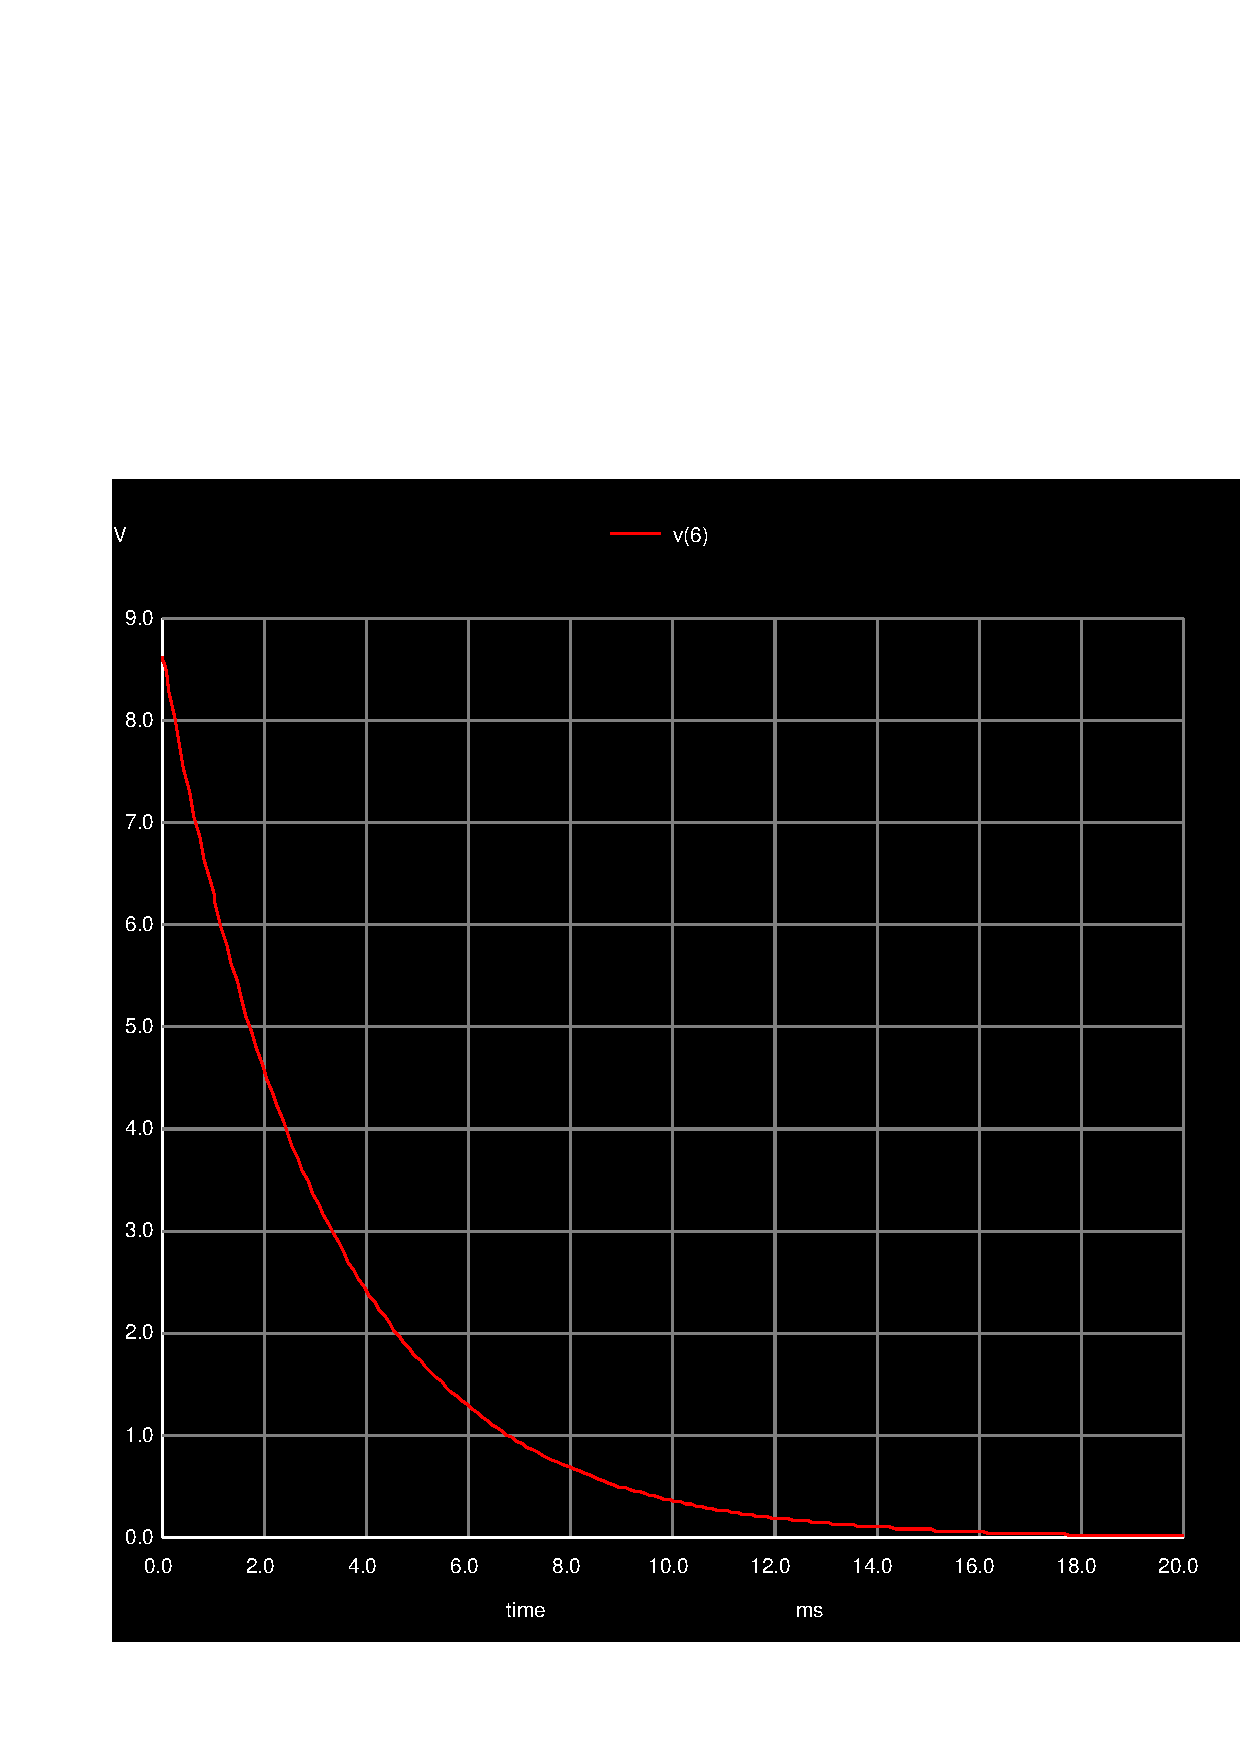
\includegraphics[width=1\linewidth]{../sim/trans3.pdf}
    \caption{RC circuit to be analysed}
    \label{fig:t2}
    \end{figure}

  \subsection{Forced response}

  \begin{table}[H]
    \centering
    \begin{tabular}{|l|r|}
      \hline    
      {\bf Name} & {\bf Value [A or V]} \\ \hline
      \input{../sim/p4_tab}
    \end{tabular}
    \caption{Operating point. A variable preceded by @ is of type {\em current}
      and expressed in Ampere; other variables are of type {\it voltage} and expressed in
      Volt.}
    \label{tab:p4}
  \end{table}

  \begin{figure}[H] \centering
    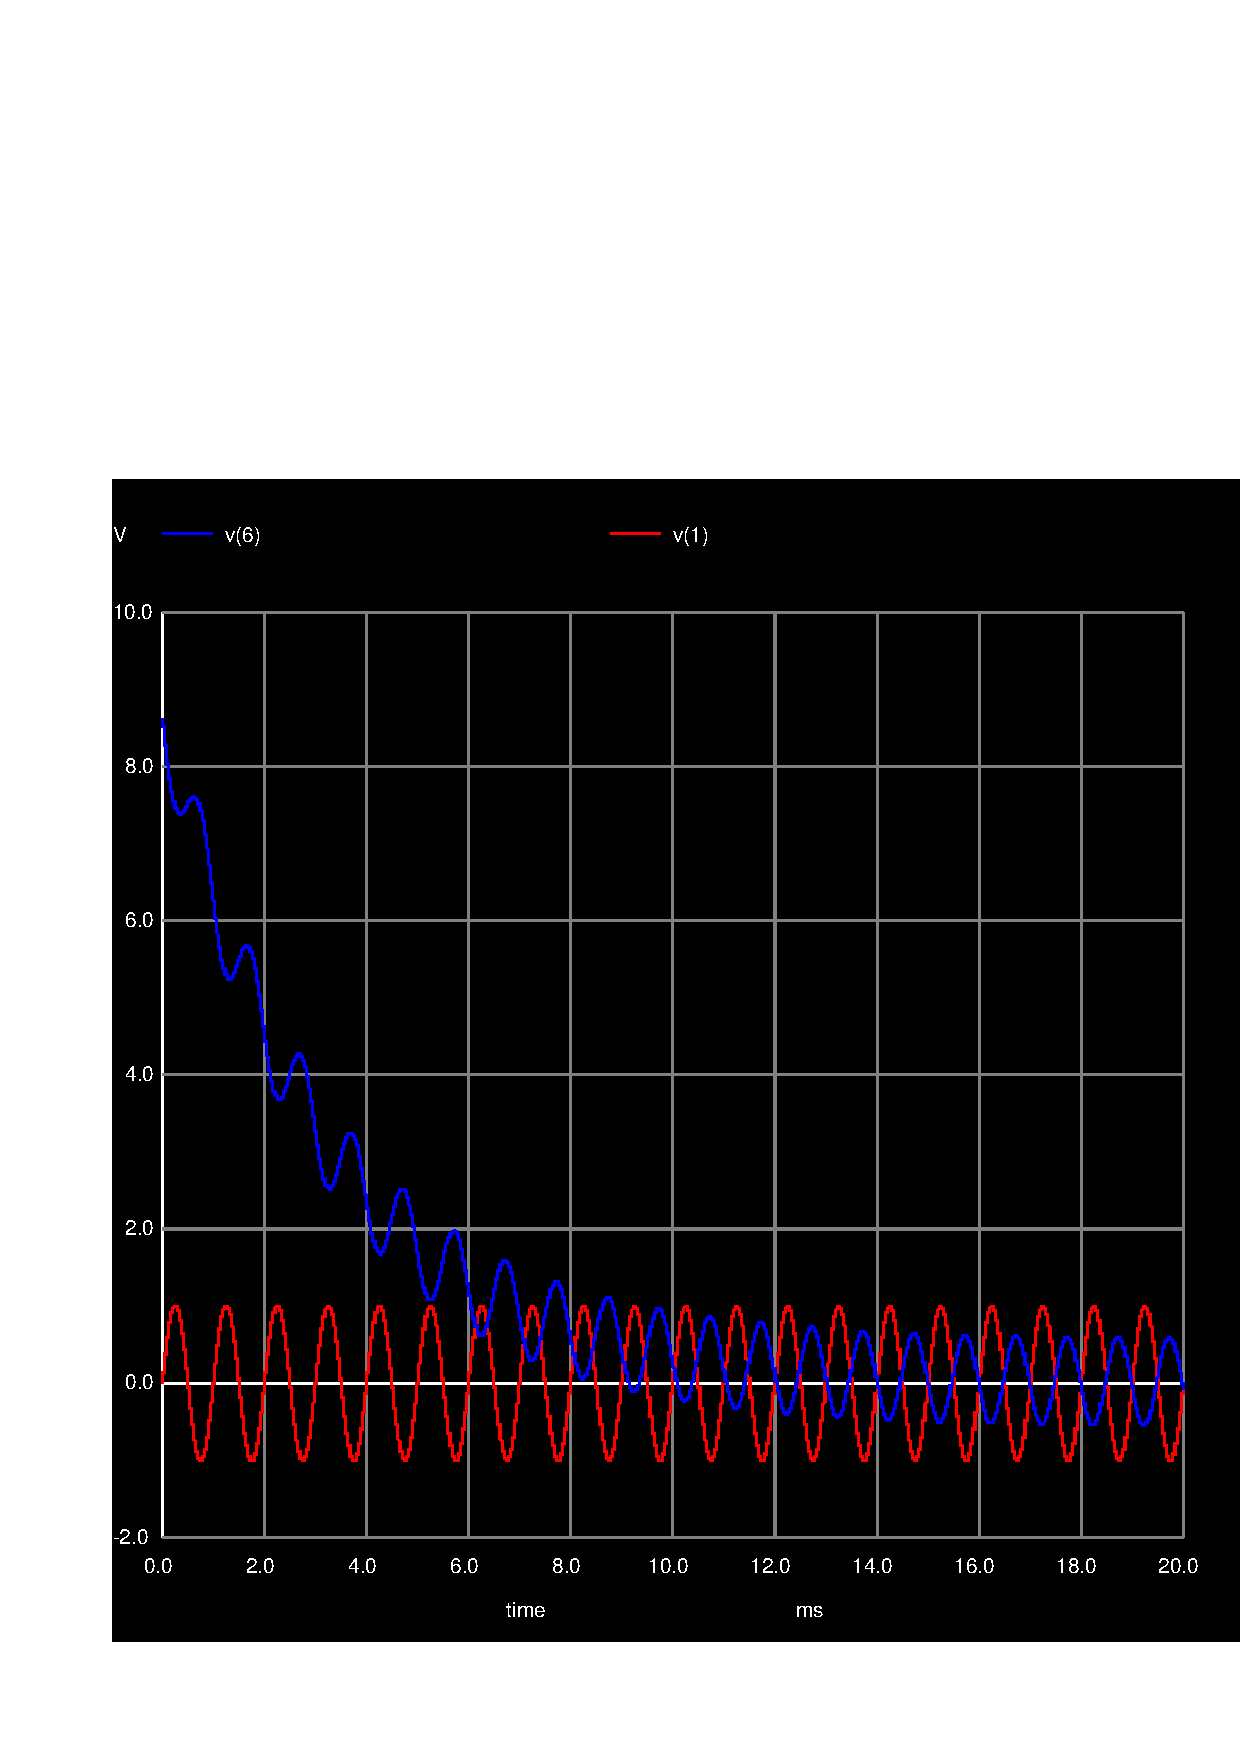
\includegraphics[width=1\linewidth]{../sim/trans4.pdf}
    \caption{RC circuit to be analysed}
    \label{fig:t2}
    \end{figure}

  \subsection{Frequency analysis}

  \begin{table}[H]
    \centering
    \begin{tabular}{|l|r|}
      \hline    
      {\bf Name} & {\bf Value [A or V]} \\ \hline
      Error(parse.c--checkvalid): @ca[i]: no such vector.\\ \hline

    \end{tabular}
    \caption{Operating point. A variable preceded by @ is of type {\em current}
      and expressed in Ampere; other variables are of type {\it voltage} and expressed in
      Volt.}
    \label{tab:p5}
  \end{table}

  \begin{figure}[H] \centering
    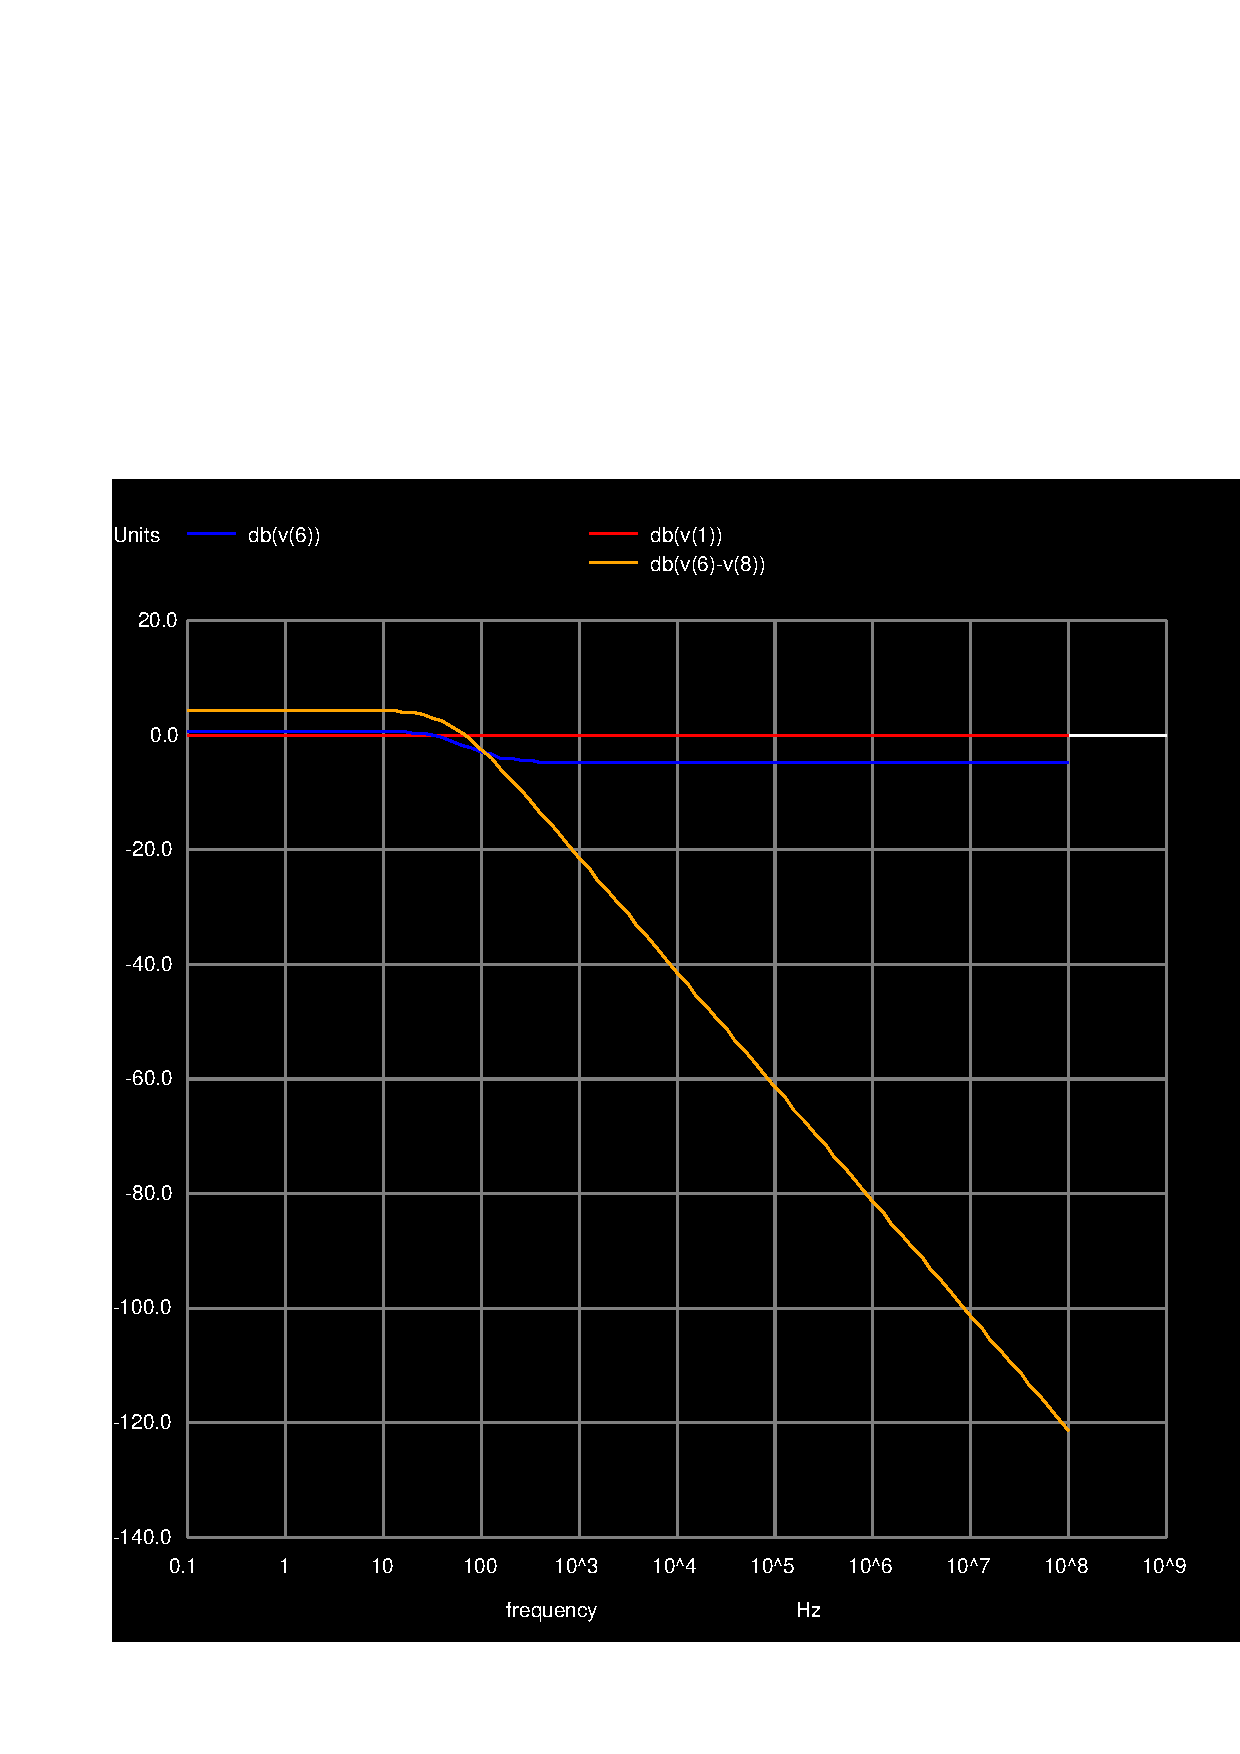
\includegraphics[width=1\linewidth]{../sim/mag5.pdf}
    \caption{RC circuit to be analysed}
    \label{fig:t2}
    \end{figure}

    \begin{figure}[H] \centering
        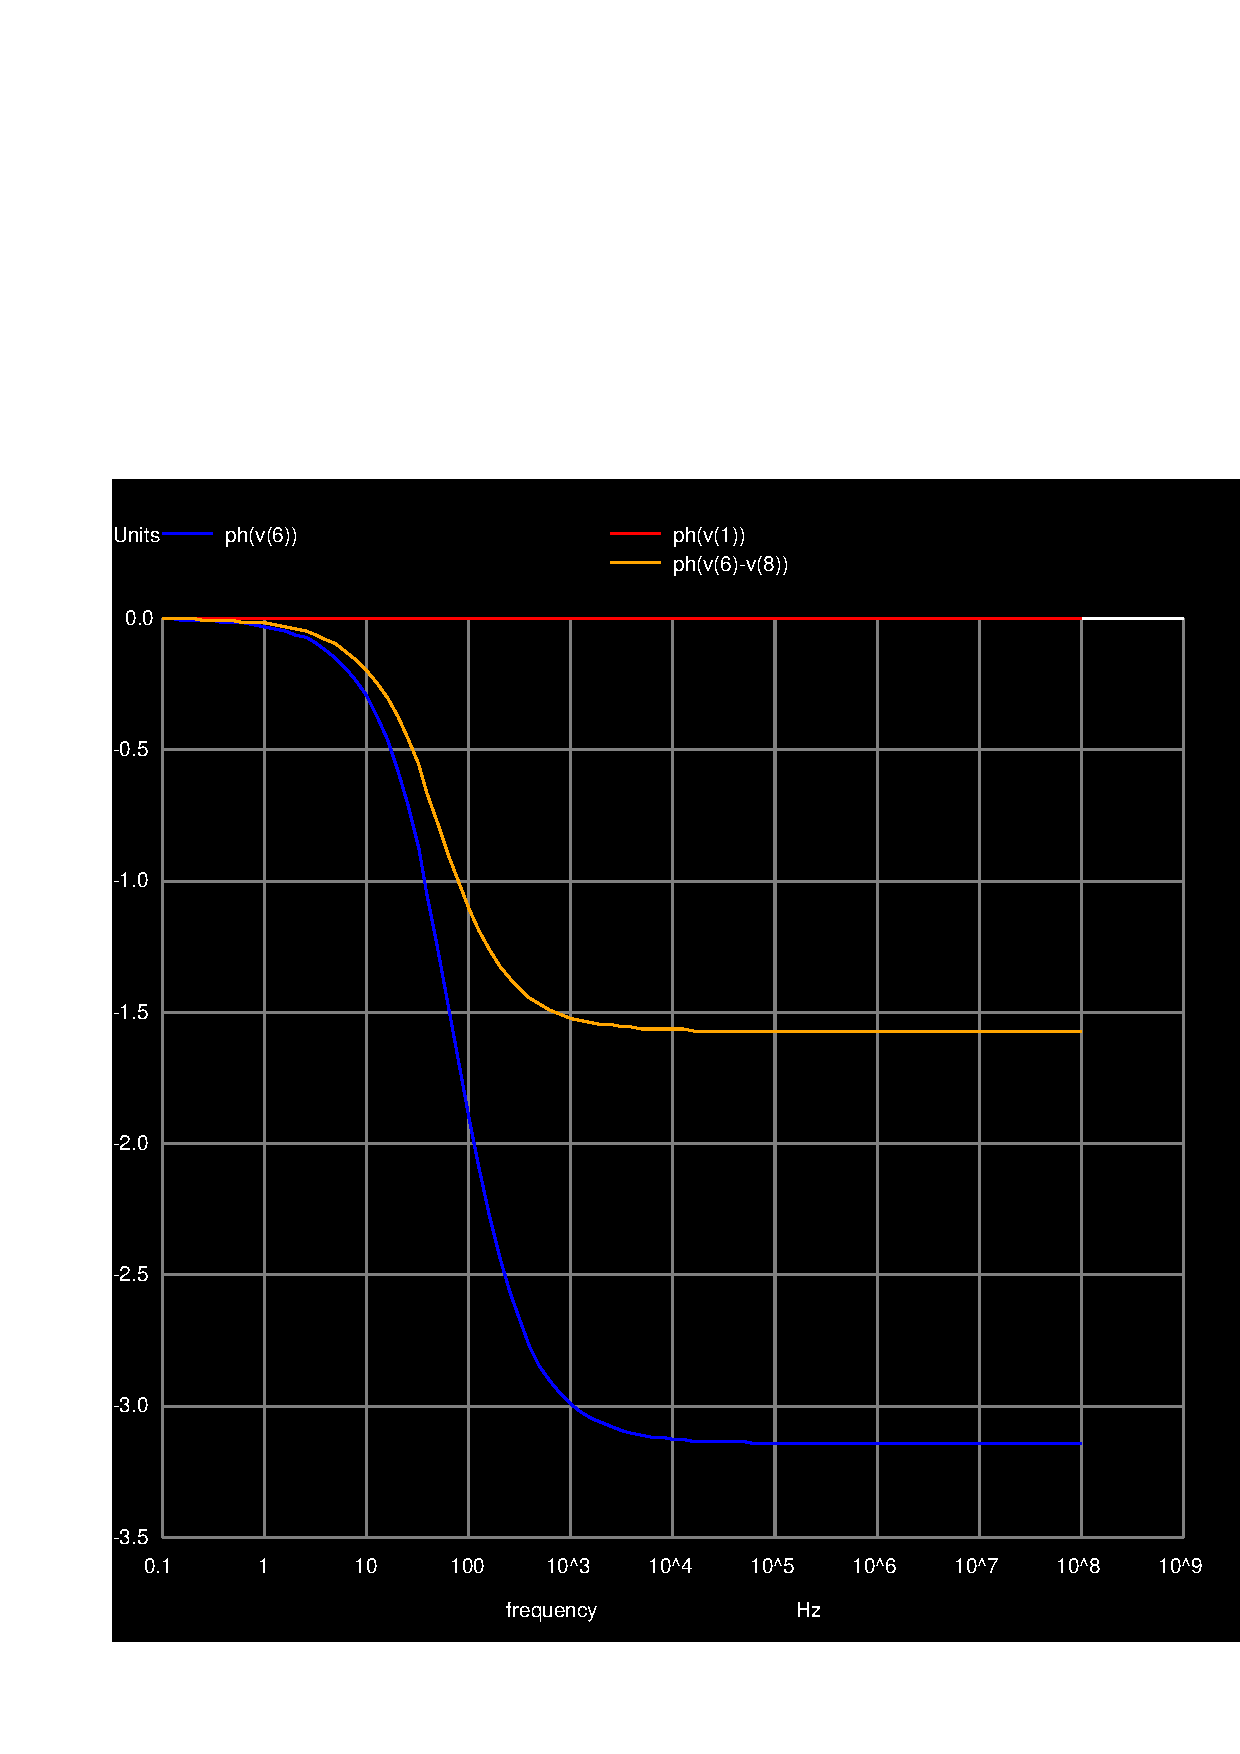
\includegraphics[width=1\linewidth]{../sim/phase5.pdf}
        \caption{RC circuit to be analysed}
        \label{fig:t2}
        \end{figure}

It should be noted that nodes G1 and G2 represent the same node G, and exist seperatly
so as to allow the measuring of current $I_c$ in ngspice, for the purpose of defining the
dependent voltage source $V_c$.

